% ============================================================
%  Compile with XeLaTeX  (Overleaf: Menu -> Settings -> Compiler -> XeLaTeX)
% ============================================================
\documentclass[12pt,a4paper]{article}

\usepackage{fontspec}
\setmainfont{TeX Gyre Termes}          % Times-like font with full Vietnamese support
\setmonofont{DejaVu Sans Mono}[Scale=0.85]
\usepackage{amsmath,amssymb}
\usepackage[margin=2.5cm]{geometry}
\usepackage{float}
\usepackage{graphicx}

% --- if an image has not been uploaded yet, show a placeholder box instead of stopping with an error ---
\let\OrigIncludegraphics\includegraphics
\renewcommand{\includegraphics}[2][]{%
  \IfFileExists{#2}{\OrigIncludegraphics[#1]{#2}}{%
    \fbox{\parbox[c][3cm][c]{0.6\linewidth}{\centering\small Missing image:\\ \texttt{\detokenize{#2}}}}}}
\usepackage{longtable,booktabs,array,calc}
\usepackage{etoolbox}
\AtBeginEnvironment{longtable}{\small}
\usepackage{caption}
\captionsetup{font=small,labelfont=bf}
\usepackage{xcolor}
\usepackage{listings}
\usepackage{setspace}
\setstretch{1.15}
\usepackage{fancyhdr}
\usepackage[hidelinks]{hyperref}

% --- helpers emitted by pandoc ---
\providecommand{\tightlist}{\setlength{\itemsep}{0pt}\setlength{\parskip}{0pt}}
\newcommand{\passthrough}[1]{#1}
\providecommand{\real}[1]{#1}
\setlength{\parindent}{0pt}
\setlength{\parskip}{6pt}
\setcounter{secnumdepth}{2}
\renewcommand{\lstlistingname}{Listing}

% --- code style ---
\lstset{
  basicstyle=\ttfamily\small,
  keywordstyle=\color{blue!60!black}\bfseries,
  commentstyle=\color{green!40!black}\itshape,
  stringstyle=\color{red!60!black},
  numbers=left, numberstyle=\tiny\color{gray}, numbersep=6pt,
  frame=single, rulecolor=\color{gray!50},
  backgroundcolor=\color{gray!5},
  breaklines=true, breakatwhitespace=false,
  columns=fullflexible, keepspaces=true,
  showstringspaces=false, captionpos=t,
  xleftmargin=1.5em, framexleftmargin=1.2em,
  extendedchars=true
}

% --- header / footer ---
\setlength{\headheight}{15pt}
\pagestyle{fancy}
\fancyhf{}
\fancyhead[L]{\small Faculty of Data Science and Artificial Intelligence}
\fancyhead[R]{\small Introduction to AI}
\fancyfoot[L]{\small Delivery Route Finding in Hanoi}
\fancyfoot[R]{\small Page \thepage}
\renewcommand{\headrulewidth}{0.4pt}

\begin{document}

% ======================= TITLE PAGE =======================
\begin{titlepage}
\centering
{\large\bfseries NATIONAL ECONOMICS UNIVERSITY\\[2pt]
COLLEGE OF TECHNOLOGY\\[2pt]
FACULTY OF DATA SCIENCE AND ARTIFICIAL INTELLIGENCE\par}
\vspace{0.8cm}

\includegraphics[width=0.28\linewidth]{figures/logo_neu.png}\par
\vspace{1cm}
{\large Introduction to Artificial Intelligence\par}
\vspace{1cm}
{\fontsize{22}{26}\selectfont\bfseries REPORT\par}
\vspace{1.2cm}
{\Large\bfseries Delivery Route Finding in Hanoi with\\[4pt] BFS, Greedy Best-First Search and A*\par}
\vspace{1.5cm}
\begin{tabular}{rl}
\textbf{Instructor:} & Dr. Trong-Nghia Nguyen\\[4pt]
\textbf{Group:} & 1
\end{tabular}
\par\vspace{0.8cm}
\begin{tabular}{clc}
\toprule
\textbf{No.} & \textbf{Full name} & \textbf{Student ID}\\
\midrule
1 & Đặng Khánh Linh & 11254245\\
2 & Hồ Đức Hải & 11252779\\
3 & Ngô Anh Tú & 11258594\\
4 & Khuất Lương Huyền Anh & 11250339\\
5 & Hà Tuấn Khôi & 31251021126\\
\bottomrule
\end{tabular}
\vfill
{\large Hanoi, October 2026\par}
\end{titlepage}


\thispagestyle{empty}
\tableofcontents
\newpage

\section*{Abstract}
\addcontentsline{toc}{section}{Abstract}

\textbf{Objective.} This report compares three search
algorithms, Breadth-First Search (BFS), Greedy Best-First
Search (GBFS) and A*, on the problem of finding a route from
a depot to each customer on a map of inner Hanoi. Two
criteria are used: path quality (total distance in km) and
search cost (number of expanded nodes).

\textbf{Methods.} The map is modelled as a graph with 12
nodes (the centroids of Hanoi's 12 urban districts) and 24
edges (pairs of adjacent districts; an edge across the Red
River is kept only when a bridge connects the two districts
directly), weighted by real road distance. The heuristic is
the Euclidean distance, which is proven to be consistent.
Uniform-Cost Search (Dijkstra) and exhaustive enumeration
serve as ground truth. Four experimental scenarios are run:
one depot with four customers, a depot placed in every
district (132 depot--customer pairs), simulated road
tortuosity, and random graphs of 25 to 800 nodes. In total,
39,952 runs were performed, all of which passed automatic
verification.

\textbf{Results.} Over the 132 depot--customer pairs, A*
finds the shortest path in 100\% of cases and expands 2.87
nodes on average, compared with 6.00 for UCS. GBFS expands
the fewest nodes (1.90) but is optimal in only 81.8\% of
cases; when it fails, its path is 17.2\% longer on average.
BFS is optimal in 84.8\% of cases; when it fails, its path
is 35.4\% longer on average. On 800-node graphs, A* expands
only 21\% of the nodes UCS does, while the optimality rate
of BFS and GBFS falls to 5\%.

\textbf{Conclusion.} A* is the most suitable algorithm for
delivery routing: it always returns the shortest path at a
low search cost. GBFS is fast but can produce substantially
longer routes, and BFS is appropriate only when all road
segments have equal length.

\textbf{Keywords:} heuristic search, A*, greedy best-first
search, breadth-first search, delivery routing, Hanoi.

\newpage
\section{Introduction}

\subsection{Context}

E-commerce in Vietnam is growing quickly, and with it the
volume of urban deliveries. The e-Conomy SEA report
projected the gross merchandise value of Vietnam's digital
economy at USD 36 billion in 2024 {[}1{]}. At this scale,
every percentage point of distance saved per order matters
for cost.

Delivering in inner Hanoi is more than finding a short line
on a map: couriers pass through narrow alleys, one-way
streets and congested areas at peak hours, and can cross the
Red River only via bridges. Once the road network is
represented as a graph, route selection becomes a search
problem in artificial intelligence, where different
algorithms yield different routes and different
computational costs.

\subsection{Problem Statement and Scope}

The assignment: given a simple map (districts, main roads),
find the shortest path from a depot to a list of customers;
apply BFS (if costs are equal), GBFS (with Euclidean
distance as the heuristic) and A*; compare the number of
expanded nodes and the paths found.

The group defines the scope as follows:

\begin{itemize}
\tightlist
\item
  Each customer is a separate route-finding problem that
  always starts from the depot; all three algorithms run on
  the same map.
\item
  BFS treats every edge as one step, matching the ``equal
  cost'' condition of the assignment; the real distance of
  the BFS path is still computed for comparison.
\item
  All roads are two-way and the map is connected.
\item
  Ordering multiple customers within one trip (the Vehicle
  Routing Problem) is out of scope and left for future work.
\end{itemize}

\subsection{Research Question and Hypotheses}

\textbf{Research question:} When finding a route from a
depot to a customer on a map of inner Hanoi, which algorithm
best balances path quality (total km) and search cost
(expanded nodes)?

\begin{longtable}[]{@{}
  >{\raggedright\arraybackslash}p{(\columnwidth - 6\tabcolsep) * \real{0.0583}}
  >{\raggedright\arraybackslash}p{(\columnwidth - 6\tabcolsep) * \real{0.3917}}
  >{\raggedright\arraybackslash}p{(\columnwidth - 6\tabcolsep) * \real{0.4083}}
  >{\raggedright\arraybackslash}p{(\columnwidth - 6\tabcolsep) * \real{0.1417}}@{}}
\caption{Research hypotheses.}\tabularnewline
\toprule\noalign{}
\begin{minipage}[b]{\linewidth}\raggedright
\end{minipage} & \begin{minipage}[b]{\linewidth}\raggedright
Hypothesis
\end{minipage} & \begin{minipage}[b]{\linewidth}\raggedright
Rationale
\end{minipage} & \begin{minipage}[b]{\linewidth}\raggedright
Tested by
\end{minipage} \\
\midrule\noalign{}
\endfirsthead
\toprule\noalign{}
\begin{minipage}[b]{\linewidth}\raggedright
\end{minipage} & \begin{minipage}[b]{\linewidth}\raggedright
Hypothesis
\end{minipage} & \begin{minipage}[b]{\linewidth}\raggedright
Rationale
\end{minipage} & \begin{minipage}[b]{\linewidth}\raggedright
Tested by
\end{minipage} \\
\midrule\noalign{}
\endhead
\bottomrule\noalign{}
\endlastfoot
H1 & BFS finds the path with the fewest edges, but not the
shortest in km & BFS is optimal only when all edges have
equal cost & KB1, KB2, KB4 \\
H2 & GBFS expands the fewest nodes but does not guarantee
optimality & GBFS considers only h(n) and ignores the
distance travelled & KB1, KB2, KB4 \\
H3 & A* always finds the shortest path and expands far fewer
nodes than UCS & The Euclidean heuristic is consistent &
KB1, KB2, KB4 \\
H4 & The more tortuous the roads relative to straight lines,
the more often BFS and GBFS fail, while A* stays optimal but
expands more nodes & The further the heuristic falls below
the true distance, the less information it carries & KB3 \\
\end{longtable}

H1--H3 follow from theory (Section 4); H4 is the group's own
addition. Scenario KB2 also serves as a robustness check: do
the conclusions depend on where the depot is placed?

\subsection{Contributions and Report Structure}

The report contributes: (i) a model of Hanoi's 12 urban
districts built from real boundary data, accounting for Red
River bridges and real road distances; (ii) a unified
measurement convention so that the expanded-node counts of
different algorithms are comparable; (iii) four experimental
scenarios with automatic verification, including a
sensitivity experiment and a scale-up experiment.

Section 2 reviews the background. Section 3 formulates the
problem and describes the data. Section 4 presents the
algorithms and measurement conventions. Section 5 walks
through the algorithms step by step on a sample map. Section
6 reports the experiments and results. Section 7 discusses
them, and Section 8 concludes.

\section{Background and Related Work}

The three algorithms in the assignment share the same
graph-search framework; they differ only in how they choose
the next node to expand {[}2{]}.

\textbf{Uninformed search.} BFS expands level by level and
returns the path with the fewest edges. Dijkstra's algorithm
{[}3{]}, or Uniform-Cost Search (UCS), expands nodes in
order of path cost g(n) and returns the shortest path when
all edge costs are positive {[}2{]}.

\textbf{Informed search.} A heuristic h(n) estimates the
remaining cost from n to the goal. GBFS uses h(n) alone. A*
uses the evaluation function f(n) = g(n) + h(n); Hart,
Nilsson and Raphael proved it optimal when the heuristic
never overestimates the true cost {[}4{]}.

\textbf{Routing under changing traffic.} When edge weights
change over time, one can search again from scratch or use
replanning methods such as D* Lite, which reuse information
from the previous search {[}5{]}.

\textbf{Multi-stop delivery.} Ordering visits to many
customers is the Vehicle Routing Problem {[}6{]}. Studies of
urban last-mile delivery often separate two levels: ordering
the stops (macro-routing) and finding the route between two
stops (micro-routing) {[}7{]}. This report addresses the
second level. Commercial mapping and delivery applications
show that routing demand is real, but one should not infer
that they rely on A* alone: real systems typically combine
several techniques.

\section{Problem Formulation and Data}

\subsection{Search Problem}

The problem is formulated with the six standard components
of a search problem {[}2{]} (Table 2), plus a heuristic for
GBFS and A*. Examples are taken from the sample map in
Section 3.3; on the 12-district map, each node is a district
centroid.

\begin{longtable}[]{@{}
  >{\raggedright\arraybackslash}p{(\columnwidth - 4\tabcolsep) * \real{0.1917}}
  >{\raggedright\arraybackslash}p{(\columnwidth - 4\tabcolsep) * \real{0.4750}}
  >{\raggedright\arraybackslash}p{(\columnwidth - 4\tabcolsep) * \real{0.3333}}@{}}
\caption{The six components of the search
problem.}\tabularnewline
\toprule\noalign{}
\begin{minipage}[b]{\linewidth}\raggedright
Component
\end{minipage} & \begin{minipage}[b]{\linewidth}\raggedright
Definition
\end{minipage} & \begin{minipage}[b]{\linewidth}\raggedright
Example on the sample map
\end{minipage} \\
\midrule\noalign{}
\endfirsthead
\toprule\noalign{}
\begin{minipage}[b]{\linewidth}\raggedright
Component
\end{minipage} & \begin{minipage}[b]{\linewidth}\raggedright
Definition
\end{minipage} & \begin{minipage}[b]{\linewidth}\raggedright
Example on the sample map
\end{minipage} \\
\midrule\noalign{}
\endhead
\bottomrule\noalign{}
\endlastfoot
State & The node where the vehicle currently is; the state
space is the set of all nodes & 11 states: S, A, B, \ldots,
J \\
Initial state & The depot & S at (0; 0) \\
Actions & Actions(n): travel along a road to an adjacent
node m, where (n, m) is an edge & Actions(S) = \{go A, go B,
go E, go H\} \\
Transition model & Result(n, go m) = m & Result(S, go E) =
E \\
Goal test & n is the node of the customer under
consideration; each run has a single goal & Routing to
customer 1 means the goal is G \\
Path cost & Sum of edge lengths, each c(n, m) \textgreater{}
0 km; BFS counts each edge as 1 while searching but still
reports real km &
S\(\rightarrow\)E\(\rightarrow\)F\(\rightarrow\)G = 4 + 5 +
8 = 17 km \\
\end{longtable}

The state only needs the current location because each run
has a single goal. If the order of multiple customers had to
be chosen, the state would also need the set of customers
already served, making the state space much larger.

\subsection{Heuristic and Consistency}

The heuristic is the straight-line distance from node n to
the customer k under consideration:

\[h(n) = \sqrt{(x_n - x_k)^2 + (y_n - y_k)^2}\]

h(k) = 0 at the goal, and h depends on the goal, so each
customer has its own table of h values. For example, on the
sample map with goal G:
\(h(F)=\sqrt{(8-10)^2+(1-0)^2}=\sqrt{5}\approx 2.24\) km.
Coordinates and road lengths must share the same unit (km)
for g(n) and h(n) to be added; on the 12-district map,
longitude and latitude are projected to the planar UTM zone
48N before computation.

\textbf{Definitions.} A heuristic is \emph{admissible} if
h(n) \(\le\) h*(n) for all n, where h*(n) is the true
minimum cost from n to the goal. A heuristic is
\emph{consistent} if h(n) \(\le\) c(n, m) + h(m) for every
edge (n, m) and h(goal) = 0; a consistent heuristic is
always admissible {[}2{]}.

\textbf{Proposition.} The Euclidean heuristic is consistent
if every edge is at least as long as the straight-line
distance between its endpoints. Indeed, for every edge (n,
m), let d denote straight-line distance and k the goal:

\[h(n) = d(n, k) \le d(n, m) + d(m, k) \le c(n, m) + h(m)\]

The first inequality is the triangle inequality; the second
uses the data condition c(n, m) \(\ge\) d(n, m). This
condition is checked in code on every edge and for every
goal before each experiment. If an edge were shorter than
the straight-line distance, h could overestimate and A*
could miss the shortest path.

\subsection{Sample Map (for Illustration)}

The group placed the nodes on a grid (1 unit = 1 km) to
deliberately create trap cases. The map has 1 depot, 10
other nodes and 15 two-way roads (Tables 3 and 4); every
edge is at least as long as its straight-line distance.

\begin{longtable}[]{@{}
  >{\raggedright\arraybackslash}p{(\columnwidth - 6\tabcolsep) * \real{0.2131}}
  >{\raggedright\arraybackslash}p{(\columnwidth - 6\tabcolsep) * \real{0.3607}}
  >{\raggedright\arraybackslash}p{(\columnwidth - 6\tabcolsep) * \real{0.2131}}
  >{\raggedright\arraybackslash}p{(\columnwidth - 6\tabcolsep) * \real{0.2131}}@{}}
\caption{Node coordinates of the sample map.}\tabularnewline
\toprule\noalign{}
\begin{minipage}[b]{\linewidth}\raggedright
Node
\end{minipage} & \begin{minipage}[b]{\linewidth}\raggedright
Role
\end{minipage} & \begin{minipage}[b]{\linewidth}\raggedright
x (km)
\end{minipage} & \begin{minipage}[b]{\linewidth}\raggedright
y (km)
\end{minipage} \\
\midrule\noalign{}
\endfirsthead
\toprule\noalign{}
\begin{minipage}[b]{\linewidth}\raggedright
Node
\end{minipage} & \begin{minipage}[b]{\linewidth}\raggedright
Role
\end{minipage} & \begin{minipage}[b]{\linewidth}\raggedright
x (km)
\end{minipage} & \begin{minipage}[b]{\linewidth}\raggedright
y (km)
\end{minipage} \\
\midrule\noalign{}
\endhead
\bottomrule\noalign{}
\endlastfoot
S & Depot & 0 & 0 \\
A & District & 5 & 6 \\
B & District & 2 & \(-2\) \\
C & District & 5 & \(-2\) \\
D & Customer 3 & 8 & \(-2\) \\
E & District & 4 & 0 \\
F & District & 8 & 1 \\
G & Customer 1 & 10 & 0 \\
H & District & 2 & 4 \\
I & Customer 2 & 8 & 5 \\
J & District & 11 & 4 \\
\end{longtable}

\begin{longtable}[]{@{}
  >{\raggedright\arraybackslash}p{(\columnwidth - 4\tabcolsep) * \real{0.0917}}
  >{\raggedright\arraybackslash}p{(\columnwidth - 4\tabcolsep) * \real{0.6500}}
  >{\raggedright\arraybackslash}p{(\columnwidth - 4\tabcolsep) * \real{0.2583}}@{}}
\caption{Edges of the sample map.}\tabularnewline
\toprule\noalign{}
\begin{minipage}[b]{\linewidth}\raggedright
Road
\end{minipage} & \begin{minipage}[b]{\linewidth}\raggedright
Real length (km)
\end{minipage} & \begin{minipage}[b]{\linewidth}\raggedright
Straight-line (km)
\end{minipage} \\
\midrule\noalign{}
\endfirsthead
\toprule\noalign{}
\begin{minipage}[b]{\linewidth}\raggedright
Road
\end{minipage} & \begin{minipage}[b]{\linewidth}\raggedright
Real length (km)
\end{minipage} & \begin{minipage}[b]{\linewidth}\raggedright
Straight-line (km)
\end{minipage} \\
\midrule\noalign{}
\endhead
\bottomrule\noalign{}
\endlastfoot
S--A & 8 & 7.81 \\
S--B & 3 & 2.83 \\
S--E & 4 & 4.00 \\
S--H & 5 & 4.47 \\
A--G & 8 & 7.81 \\
A--H & 4 & 3.61 \\
A--I & 4 & 3.16 \\
B--C & 3 & 3.00 \\
C--D & 3 & 3.00 \\
D--G & 3 & 2.83 \\
E--F & 5 & 4.12 \\
F--G & 8 & 2.24 \\
F--I & 4 & 4.00 \\
I--J & 4 & 3.16 \\
J--G & 5 & 4.12 \\
\end{longtable}

The three customers each illustrate one point:

\begin{itemize}
\tightlist
\item
  \textbf{Customer 1 = G} contains both traps. The BFS trap:
  S\(\rightarrow\)A\(\rightarrow\)G has only 2 edges but is
  16 km long, while
  S\(\rightarrow\)B\(\rightarrow\)C\(\rightarrow\)D\(\rightarrow\)G
  has 4 edges and is only 12 km. The GBFS trap: F is only
  2.24 km from G as the crow flies, but the F--G road is 8
  km (simulating a detour to a bridge).
\item
  \textbf{Customer 2 = I} is the control case: all three
  algorithms find the shortest path.
\item
  \textbf{Customer 3 = D} has two 3-edge paths,
  S\(\rightarrow\)A\(\rightarrow\)G\(\rightarrow\)D (19 km)
  and S\(\rightarrow\)B\(\rightarrow\)C\(\rightarrow\)D (9
  km); the tie-breaking order decides which one BFS returns.
\end{itemize}

\subsection{The 12-District Map of Hanoi (for
Experiments)}

\textbf{Data source.} The boundaries of the 12 districts
come from the dvhcvn dataset {[}8{]} (data date 1 March
2025) and were cross-checked against geoBoundaries {[}9{]}.
Boundaries are projected to UTM zone 48N; each district's
node is the geometric centroid of its polygon; two districts
are adjacent if they share a boundary longer than 300 m.
Centroids computed from the two sources differ by at most
0.143 km, and planar UTM distances differ from geodesic
distances by at most 3 m. The 12 centroids are listed in
Appendix A; the map is shown in Figure 1.

\textbf{Administrative note.} These are the boundaries
before 1 July 2025, when the district level still existed;
``district'' in this report denotes a geographic area used
to build the graph, not a current administrative unit.

\textbf{Red River crossings.} Of the 12 districts, only Long
Biên lies on the east bank of the Red River. Two districts
adjacent across the river are connected only if a bridge
links them directly (Table 5), so 2 of the 5 pairs are
removed and the graph keeps 24 edges.

\begin{longtable}[]{@{}
  >{\raggedright\arraybackslash}p{(\columnwidth - 4\tabcolsep) * \real{0.2833}}
  >{\raggedright\arraybackslash}p{(\columnwidth - 4\tabcolsep) * \real{0.5667}}
  >{\raggedright\arraybackslash}p{(\columnwidth - 4\tabcolsep) * \real{0.1500}}@{}}
\caption{District pairs adjacent across the Red
River.}\tabularnewline
\toprule\noalign{}
\begin{minipage}[b]{\linewidth}\raggedright
District pair
\end{minipage} & \begin{minipage}[b]{\linewidth}\raggedright
Direct bridge
\end{minipage} & \begin{minipage}[b]{\linewidth}\raggedright
Decision
\end{minipage} \\
\midrule\noalign{}
\endfirsthead
\toprule\noalign{}
\begin{minipage}[b]{\linewidth}\raggedright
District pair
\end{minipage} & \begin{minipage}[b]{\linewidth}\raggedright
Direct bridge
\end{minipage} & \begin{minipage}[b]{\linewidth}\raggedright
Decision
\end{minipage} \\
\midrule\noalign{}
\endhead
\bottomrule\noalign{}
\endlastfoot
Hoàn Kiếm -- Long Biên & Long Biên Bridge {[}11{]}, Chương
Dương Bridge {[}10{]} & Keep \\
Hai Bà Trưng -- Long Biên & Vĩnh Tuy Bridge {[}10{]} &
Keep \\
Hoàng Mai -- Long Biên & Thanh Trì Bridge {[}11{]} & Keep \\
Ba Đình -- Long Biên & None & Remove \\
Tây Hồ -- Long Biên & None; Nhật Tân Bridge links Tây Hồ to
Đông Anh {[}10{]} & Remove \\
\end{longtable}

\begin{figure}[H]
\centering
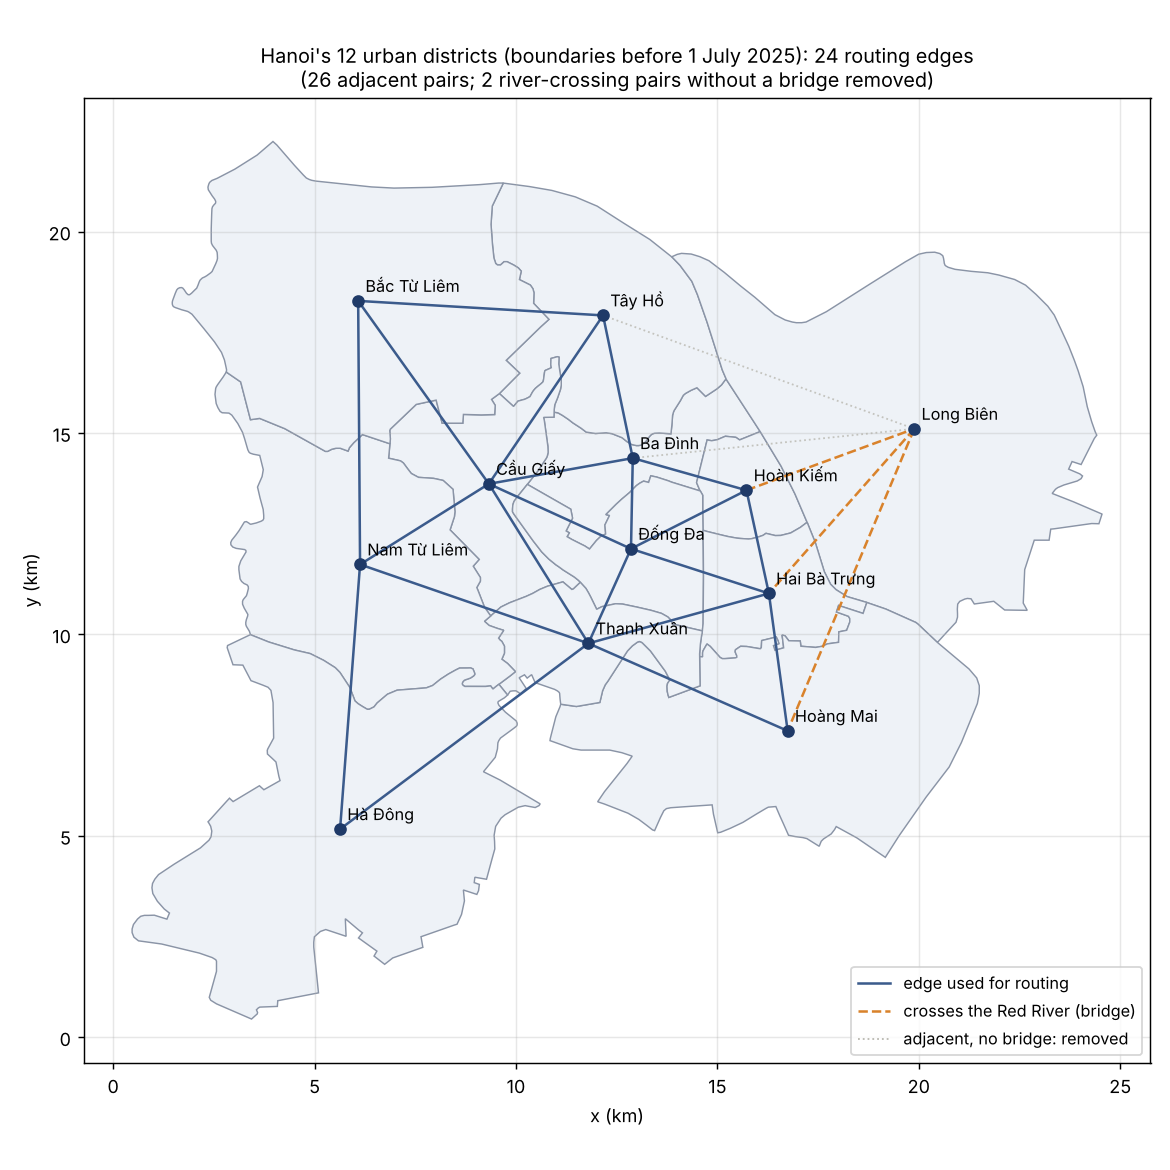
\includegraphics[width=0.75\linewidth,height=0.7\textheight,keepaspectratio]{figures/hanoi_12_quan_ban_do.png}
\caption{The 12 districts of Hanoi: centroids, the 24 edges used for routing, the 3 river crossings with bridges (dashed) and the 2 removed pairs (dotted).}
\end{figure}

\textbf{Edge lengths.} Real road distances were looked up on
Google Maps. For 20 of the 24 edges, the measured value is
used directly; for these, the road distance is 1.16--2.36
times the straight-line distance, with a median of about
1.5. Four edges were measured shorter than the straight-line
distance between the two centroids, because they were
measured between points other than the centroids; to
preserve the consistency condition of Section 3.2, these
four edges are raised to their straight-line distance (Table
6). All 24 edges are listed in Appendix B.

\begin{longtable}[]{@{}
  >{\raggedright\arraybackslash}p{(\columnwidth - 4\tabcolsep) * \real{0.4380}}
  >{\raggedright\arraybackslash}p{(\columnwidth - 4\tabcolsep) * \real{0.1818}}
  >{\raggedright\arraybackslash}p{(\columnwidth - 4\tabcolsep) * \real{0.3802}}@{}}
\caption{Edges raised to the straight-line
distance.}\tabularnewline
\toprule\noalign{}
\begin{minipage}[b]{\linewidth}\raggedright
Edge
\end{minipage} & \begin{minipage}[b]{\linewidth}\raggedright
Measured (km)
\end{minipage} & \begin{minipage}[b]{\linewidth}\raggedright
Used in experiments (km)
\end{minipage} \\
\midrule\noalign{}
\endfirsthead
\toprule\noalign{}
\begin{minipage}[b]{\linewidth}\raggedright
Edge
\end{minipage} & \begin{minipage}[b]{\linewidth}\raggedright
Measured (km)
\end{minipage} & \begin{minipage}[b]{\linewidth}\raggedright
Used in experiments (km)
\end{minipage} \\
\midrule\noalign{}
\endhead
\bottomrule\noalign{}
\endlastfoot
Ba Đình -- Hoàn Kiếm & 1.8 & 2.933 \\
Hoàn Kiếm -- Hai Bà Trưng & 2.5 & 2.622 \\
Thanh Xuân -- Hà Đông & 4.5 & 7.698 \\
Nam Từ Liêm -- Hà Đông & 5.1 & 6.589 \\
\end{longtable}

\section{Algorithms and Measurement Conventions}

\subsection{Common Search Framework}

The three algorithms differ only in how they order the
frontier, the list of nodes waiting to be expanded
(Algorithm 1, Table 7). Of the three, A* is the only one
guaranteed to find the shortest path on a weighted map. UCS
is run as the ground truth.

\begin{lstlisting}[caption={Graph search framework}]
FIND_PATH(depot, goal):
    frontier ← {depot};  parent[depot] ← none
    while frontier is not empty:
        n ← remove the highest-priority node from frontier
        if n = goal: return the path rebuilt from parent[]
        mark n as expanded               # counts 1 expanded node
        for each neighbour m of n (in a fixed order):
            if m not yet seen (A*/UCS: or a smaller g(m) is found):
                parent[m] ← n;  add m to frontier
    return failure
\end{lstlisting}

\begin{longtable}[]{@{}
  >{\raggedright\arraybackslash}p{(\columnwidth - 6\tabcolsep) * \real{0.2083}}
  >{\raggedright\arraybackslash}p{(\columnwidth - 6\tabcolsep) * \real{0.3917}}
  >{\raggedright\arraybackslash}p{(\columnwidth - 6\tabcolsep) * \real{0.2000}}
  >{\raggedright\arraybackslash}p{(\columnwidth - 6\tabcolsep) * \real{0.2000}}@{}}
\caption{How each algorithm chooses the ``highest-priority''
node.}\tabularnewline
\toprule\noalign{}
\begin{minipage}[b]{\linewidth}\raggedright
Algorithm
\end{minipage} & \begin{minipage}[b]{\linewidth}\raggedright
``Highest priority'' means
\end{minipage} & \begin{minipage}[b]{\linewidth}\raggedright
Uses edge lengths?
\end{minipage} & \begin{minipage}[b]{\linewidth}\raggedright
Uses heuristic?
\end{minipage} \\
\midrule\noalign{}
\endfirsthead
\toprule\noalign{}
\begin{minipage}[b]{\linewidth}\raggedright
Algorithm
\end{minipage} & \begin{minipage}[b]{\linewidth}\raggedright
``Highest priority'' means
\end{minipage} & \begin{minipage}[b]{\linewidth}\raggedright
Uses edge lengths?
\end{minipage} & \begin{minipage}[b]{\linewidth}\raggedright
Uses heuristic?
\end{minipage} \\
\midrule\noalign{}
\endhead
\bottomrule\noalign{}
\endlastfoot
BFS & Entered the frontier earliest (FIFO queue) & No &
No \\
GBFS & Smallest h(n) & No & Yes \\
A* & Smallest f(n) = g(n) + h(n) & Yes & Yes \\
UCS (ground truth) & Smallest g(n), i.e.~A* with h = 0 & Yes
& No \\
\end{longtable}

\subsection{Theoretical Properties}

\begin{longtable}[]{@{}
  >{\raggedright\arraybackslash}p{(\columnwidth - 6\tabcolsep) * \real{0.1750}}
  >{\raggedright\arraybackslash}p{(\columnwidth - 6\tabcolsep) * \real{0.2917}}
  >{\raggedright\arraybackslash}p{(\columnwidth - 6\tabcolsep) * \real{0.2917}}
  >{\raggedright\arraybackslash}p{(\columnwidth - 6\tabcolsep) * \real{0.2417}}@{}}
\caption{Completeness, optimality and complexity
{[}2{]}.}\tabularnewline
\toprule\noalign{}
\begin{minipage}[b]{\linewidth}\raggedright
Algorithm
\end{minipage} & \begin{minipage}[b]{\linewidth}\raggedright
Complete?
\end{minipage} & \begin{minipage}[b]{\linewidth}\raggedright
Optimal?
\end{minipage} & \begin{minipage}[b]{\linewidth}\raggedright
Time and space
\end{minipage} \\
\midrule\noalign{}
\endfirsthead
\toprule\noalign{}
\begin{minipage}[b]{\linewidth}\raggedright
Algorithm
\end{minipage} & \begin{minipage}[b]{\linewidth}\raggedright
Complete?
\end{minipage} & \begin{minipage}[b]{\linewidth}\raggedright
Optimal?
\end{minipage} & \begin{minipage}[b]{\linewidth}\raggedright
Time and space
\end{minipage} \\
\midrule\noalign{}
\endhead
\bottomrule\noalign{}
\endlastfoot
BFS & Yes, if the branching factor is finite & Only if all
edges have equal cost & \(O(b^d)\) \\
GBFS & Yes for graph search on a finite graph & No & Worst
case \(O(b^m)\); far less with a good heuristic \\
A* & Yes, if the branching factor is finite and every edge
cost \(\ge\) \(\varepsilon\) \textgreater{} 0 & Yes, if h is
admissible (tree search) or consistent (graph search) &
Worst case \(O(b^d)\); memory is the main weakness \\
UCS & Yes, if every edge cost \(\ge\) \(\varepsilon\)
\textgreater{} 0 & Yes &
\(O(b^{1+\lfloor C^*/\varepsilon\rfloor})\) \\
\end{longtable}

Here b is the branching factor, d the depth of the
shallowest solution, m the maximum depth and C* the cost of
the optimal path. On a graph with V nodes and E edges and a
visited set, BFS runs in O(V + E); GBFS, A* and UCS with a
heap run in O((V + E) log V).

\textbf{Relationship between A* and UCS.} With a consistent
h, A* expands only nodes with g(n) + h(n) \(\le\) C*,
i.e.~g(n) \(\le\) C* \(-\) h(n) \(\le\) C*. Every such node
also lies in the region UCS must explore, so A* never
expands more nodes than UCS (up to ties at exactly C*). The
closer h is to h*, the fewer nodes A* expands; if h = h*, A*
expands only the nodes on the optimal path.

\subsection{Measurement Conventions}

All four algorithms follow the same conventions (Table 9);
otherwise their expanded-node counts would not be
comparable.

\begin{longtable}[]{@{}
  >{\raggedright\arraybackslash}p{(\columnwidth - 4\tabcolsep) * \real{0.2314}}
  >{\raggedright\arraybackslash}p{(\columnwidth - 4\tabcolsep) * \real{0.3967}}
  >{\raggedright\arraybackslash}p{(\columnwidth - 4\tabcolsep) * \real{0.3719}}@{}}
\caption{Shared measurement conventions.}\tabularnewline
\toprule\noalign{}
\begin{minipage}[b]{\linewidth}\raggedright
Convention
\end{minipage} & \begin{minipage}[b]{\linewidth}\raggedright
Group's choice
\end{minipage} & \begin{minipage}[b]{\linewidth}\raggedright
Reason
\end{minipage} \\
\midrule\noalign{}
\endfirsthead
\toprule\noalign{}
\begin{minipage}[b]{\linewidth}\raggedright
Convention
\end{minipage} & \begin{minipage}[b]{\linewidth}\raggedright
Group's choice
\end{minipage} & \begin{minipage}[b]{\linewidth}\raggedright
Reason
\end{minipage} \\
\midrule\noalign{}
\endhead
\bottomrule\noalign{}
\endlastfoot
Expanded node & A node removed from the frontier whose
neighbours are generated; the goal node and stale A* entries
are not counted & Measures exactly the work the algorithm
does \\
Goal test timing & When a node is removed from the frontier
& For A*, testing at generation can return a suboptimal path
(Section 5.4) \\
Graph search & BFS and GBFS keep the set of seen nodes; A*
keeps the best g of each node and the set of expanded nodes
& Two-way roads would make tree search loop forever \\
A* finds a better path & Update g and parent, push a new
entry onto the heap; skip stale entries when popped; never
reopen an expanded node & With a consistent heuristic, an
expanded node already has its best path \\
Tie-breaking & A fixed node order: alphabetical on the
sample map, administrative code on the 12-district map &
Results are reproducible and easy to check by hand \\
\end{longtable}

Tie-breaking does not change the number of edges in the BFS
path but can change its length. For customer 3 = D on the
sample map, A precedes B, so BFS returns
S\(\rightarrow\)A\(\rightarrow\)G\(\rightarrow\)D (19 km);
with the reverse order, BFS would return
S\(\rightarrow\)B\(\rightarrow\)C\(\rightarrow\)D (9 km).

\subsection{Verification}

Every run is checked automatically: (1) the path is valid:
it starts at the depot, ends at the goal, every step is a
real edge and no node repeats; (2) the total km recomputed
edge by edge matches the km accumulated by the algorithm;
(3) against exhaustive enumeration of all simple paths: BFS
must have the fewest edges, A* and UCS must have the
shortest total km, and GBFS must produce the same expansion
order as a second, independently written implementation. On
large graphs (KB4), exhaustive enumeration is infeasible, so
UCS is the ground truth.

\section{Step-by-Step Illustration}

This section runs the three algorithms for customer 1 = G on
the sample map. For the same customer, the three algorithms
return three different paths: BFS 16 km (5 expanded nodes),
GBFS 17 km (3 nodes), A* 12 km (6 nodes). UCS also finds 12
km but expands 8 nodes. The tables below were generated by
code under the conventions of Section 4.3; the last column
lists the frontier in the order nodes will be removed, with
their priority values.

\begin{lstlisting}[language=Python, caption={Shared helper.}]
def build_path(parent, goal):
    # Rebuild the path by following parent links back from the goal
    path = [goal]
    while parent[path[-1]] is not None:
        path.append(parent[path[-1]])
    return path[::-1]
\end{lstlisting}

\subsection{BFS}

\begin{lstlisting}[language=Python, caption={BFS implementation.}]
def bfs(G, depot, goal):
    frontier = deque([depot])
    parent = {depot: None}  # also serves as the set of seen nodes
    g = {depot: 0.0}        # km travelled, for verification only
    expanded, generated, max_frontier = [], 1, 1
    while frontier:
        n = frontier.popleft()                 # FIFO: oldest node first
        if n == goal:                          # goal test on removal
            return make_result(build_path(parent, goal), expanded, generated, max_frontier, g[goal])
        expanded.append(n)                     # count one expanded node
        for m in G.neighbors[n]:
            if m not in parent:                # graph search: skip seen nodes
                parent[m], g[m] = n, g[n] + G.cost(n, m)
                frontier.append(m)
                generated += 1
        max_frontier = max(max_frontier, len(frontier))
    return make_result(None, expanded, generated, max_frontier, math.nan)
\end{lstlisting}

BFS never reads the edge length when choosing a node;
\passthrough{\lstinline!G.cost(n, m)!} is only accumulated
so that the real km of the returned path can be reported and
verified.

\begin{longtable}[]{@{}
  >{\raggedright\arraybackslash}p{(\columnwidth - 6\tabcolsep) * \real{0.0909}}
  >{\raggedright\arraybackslash}p{(\columnwidth - 6\tabcolsep) * \real{0.1405}}
  >{\raggedright\arraybackslash}p{(\columnwidth - 6\tabcolsep) * \real{0.3140}}
  >{\raggedright\arraybackslash}p{(\columnwidth - 6\tabcolsep) * \real{0.4545}}@{}}
\caption{BFS for customer 1: S \(\rightarrow\) A
\(\rightarrow\) G = 16 km, 5 expanded nodes.}\tabularnewline
\toprule\noalign{}
\begin{minipage}[b]{\linewidth}\raggedright
Step
\end{minipage} & \begin{minipage}[b]{\linewidth}\raggedright
Removed
\end{minipage} & \begin{minipage}[b]{\linewidth}\raggedright
New neighbours added
\end{minipage} & \begin{minipage}[b]{\linewidth}\raggedright
Frontier after step (FIFO)
\end{minipage} \\
\midrule\noalign{}
\endfirsthead
\toprule\noalign{}
\begin{minipage}[b]{\linewidth}\raggedright
Step
\end{minipage} & \begin{minipage}[b]{\linewidth}\raggedright
Removed
\end{minipage} & \begin{minipage}[b]{\linewidth}\raggedright
New neighbours added
\end{minipage} & \begin{minipage}[b]{\linewidth}\raggedright
Frontier after step (FIFO)
\end{minipage} \\
\midrule\noalign{}
\endhead
\bottomrule\noalign{}
\endlastfoot
1 & S & A, B, E, H & A, B, E, H \\
2 & A & G, I & B, E, H, G, I \\
3 & B & C & E, H, G, I, C \\
4 & E & F & H, G, I, C, F \\
5 & H & (none) & G, I, C, F \\
6 & G & Goal: stop & \\
\end{longtable}

G enters the frontier as early as step 2 via A, so BFS
returns the 2-edge path S\(\rightarrow\)A\(\rightarrow\)G
even though it is 16 km long.

\subsection{GBFS}

\begin{lstlisting}[language=Python, caption={GBFS implementation.}]
def gbfs(G, depot, goal):
    frontier = [(G.h(depot, goal), G.key[depot], depot)]   # heap ordered by (h, tie-break key)
    parent = {depot: None}
    g = {depot: 0.0}        # km travelled, for verification only
    expanded, generated, max_frontier = [], 1, 1
    while frontier:
        _, _, n = heapq.heappop(frontier)      # node with the smallest h(n)
        if n == goal:                          # goal test on removal
            return make_result(build_path(parent, goal), expanded, generated, max_frontier, g[goal])
        expanded.append(n)
        for m in G.neighbors[n]:
            if m not in parent:                # graph search: skip seen nodes
                parent[m], g[m] = n, g[n] + G.cost(n, m)
                heapq.heappush(frontier, (G.h(m, goal), G.key[m], m))
                generated += 1
        max_frontier = max(max_frontier, len(frontier))
    return make_result(None, expanded, generated, max_frontier, math.nan)
\end{lstlisting}

The only difference from BFS is the frontier: a priority
queue keyed by h(n) instead of a FIFO queue. Like BFS, GBFS
never uses the distance already travelled to choose a node.

\begin{longtable}[]{@{}
  >{\raggedright\arraybackslash}p{(\columnwidth - 6\tabcolsep) * \real{0.0917}}
  >{\raggedright\arraybackslash}p{(\columnwidth - 6\tabcolsep) * \real{0.1417}}
  >{\raggedright\arraybackslash}p{(\columnwidth - 6\tabcolsep) * \real{0.3500}}
  >{\raggedright\arraybackslash}p{(\columnwidth - 6\tabcolsep) * \real{0.4167}}@{}}
\caption{GBFS for customer 1: S \(\rightarrow\) E
\(\rightarrow\) F \(\rightarrow\) G = 17 km, 3 expanded
nodes.}\tabularnewline
\toprule\noalign{}
\begin{minipage}[b]{\linewidth}\raggedright
Step
\end{minipage} & \begin{minipage}[b]{\linewidth}\raggedright
Removed (h)
\end{minipage} & \begin{minipage}[b]{\linewidth}\raggedright
New neighbours (h)
\end{minipage} & \begin{minipage}[b]{\linewidth}\raggedright
Frontier after step, by h
\end{minipage} \\
\midrule\noalign{}
\endfirsthead
\toprule\noalign{}
\begin{minipage}[b]{\linewidth}\raggedright
Step
\end{minipage} & \begin{minipage}[b]{\linewidth}\raggedright
Removed (h)
\end{minipage} & \begin{minipage}[b]{\linewidth}\raggedright
New neighbours (h)
\end{minipage} & \begin{minipage}[b]{\linewidth}\raggedright
Frontier after step, by h
\end{minipage} \\
\midrule\noalign{}
\endhead
\bottomrule\noalign{}
\endlastfoot
1 & S (10.00) & A (7.81), B (8.25), E (6.00), H (8.94) & E
6.00 \(\cdot\) A 7.81 \(\cdot\) B 8.25 \(\cdot\) H 8.94 \\
2 & E (6.00) & F (2.24) & F 2.24 \(\cdot\) A 7.81 \(\cdot\)
B 8.25 \(\cdot\) H 8.94 \\
3 & F (2.24) & G (0.00), I (5.39) & G 0.00 \(\cdot\) I 5.39
\(\cdot\) A 7.81 \(\cdot\) B 8.25 \(\cdot\) H 8.94 \\
4 & G (0.00) & Goal: stop & \\
\end{longtable}

F looks very close to G (2.24 km as the crow flies), so GBFS
rushes to F and then takes the 8 km F--G road: the fewest
nodes, but the longest path.

\subsection{A*}

\begin{lstlisting}[language=Python, caption={A* implementation (UCS is the same function with `use\_heuristic=False`, i.e. h = 0).}]
def a_star(G, depot, goal, use_heuristic=True):
    h = (lambda n: G.h(n, goal)) if use_heuristic else (lambda n: 0.0)
    g = {depot: 0.0}                           # best known cost to each node
    parent = {depot: None}
    frontier = [(h(depot), G.key[depot], depot)]   # heap ordered by (f, tie-break key)
    closed = set()                             # expanded nodes
    expanded, generated, max_frontier = [], 1, 1
    while frontier:
        _, _, n = heapq.heappop(frontier)      # node with the smallest f = g + h
        if n in closed:
            continue                           # stale entry: a better path was found later
        if n == goal:                          # goal test on removal
            return make_result(build_path(parent, goal), expanded, generated, max_frontier, g[goal])
        closed.add(n)
        expanded.append(n)
        for m in G.neighbors[n]:
            if m in closed:
                continue                       # never reopen an expanded node
            new_g = g[n] + G.cost(n, m)
            if m not in g or new_g < g[m] - EPS:
                g[m], parent[m] = new_g, n     # better path: update g and parent
                heapq.heappush(frontier, (new_g + h(m), G.key[m], m))
                generated += 1
        max_frontier = max(max_frontier, len(frontier))
    return make_result(None, expanded, generated, max_frontier, math.nan)


def ucs(G, depot, goal):
    # UCS (Dijkstra) is A* with h = 0
    return a_star(G, depot, goal, use_heuristic=False)
\end{lstlisting}

Three details implement the conventions of Table 9: the goal
is tested when a node is popped, not when it is generated; a
better path to a node pushes a new heap entry instead of
editing the old one; and stale entries are skipped when
popped. \passthrough{\lstinline!EPS!} (\(10^{-9}\)) guards
against floating-point noise when comparing costs.

\begin{longtable}[]{@{}
  >{\raggedright\arraybackslash}p{(\columnwidth - 6\tabcolsep) * \real{0.0917}}
  >{\raggedright\arraybackslash}p{(\columnwidth - 6\tabcolsep) * \real{0.1583}}
  >{\raggedright\arraybackslash}p{(\columnwidth - 6\tabcolsep) * \real{0.3833}}
  >{\raggedright\arraybackslash}p{(\columnwidth - 6\tabcolsep) * \real{0.3667}}@{}}
\caption{A* for customer 1: S \(\rightarrow\) B
\(\rightarrow\) C \(\rightarrow\) D \(\rightarrow\) G = 12
km, 6 expanded nodes.}\tabularnewline
\toprule\noalign{}
\begin{minipage}[b]{\linewidth}\raggedright
Step
\end{minipage} & \begin{minipage}[b]{\linewidth}\raggedright
Removed (g; f)
\end{minipage} & \begin{minipage}[b]{\linewidth}\raggedright
New or updated neighbours (g; f)
\end{minipage} & \begin{minipage}[b]{\linewidth}\raggedright
Frontier after step, by f
\end{minipage} \\
\midrule\noalign{}
\endfirsthead
\toprule\noalign{}
\begin{minipage}[b]{\linewidth}\raggedright
Step
\end{minipage} & \begin{minipage}[b]{\linewidth}\raggedright
Removed (g; f)
\end{minipage} & \begin{minipage}[b]{\linewidth}\raggedright
New or updated neighbours (g; f)
\end{minipage} & \begin{minipage}[b]{\linewidth}\raggedright
Frontier after step, by f
\end{minipage} \\
\midrule\noalign{}
\endhead
\bottomrule\noalign{}
\endlastfoot
1 & S (0; 10.00) & A (8; 15.81), B (3; 11.25), E (4; 10.00),
H (5; 13.94) & E 10.00 \(\cdot\) B 11.25 \(\cdot\) H 13.94
\(\cdot\) A 15.81 \\
2 & E (4; 10.00) & F (9; 11.24) & F 11.24 \(\cdot\) B 11.25
\(\cdot\) H 13.94 \(\cdot\) A 15.81 \\
3 & F (9; 11.24) & G (17; 17.00), I (13; 18.39) & B 11.25
\(\cdot\) H 13.94 \(\cdot\) A 15.81 \(\cdot\) G 17.00
\(\cdot\) I 18.39 \\
4 & B (3; 11.25) & C (6; 11.39) & C 11.39 \(\cdot\) H 13.94
\(\cdot\) A 15.81 \(\cdot\) G 17.00 \(\cdot\) I 18.39 \\
5 & C (6; 11.39) & D (9; 11.83) & D 11.83 \(\cdot\) H 13.94
\(\cdot\) A 15.81 \(\cdot\) G 17.00 \(\cdot\) I 18.39 \\
6 & D (9; 11.83) & G updated: g 17 \(\rightarrow\) 12, f =
12.00 & G 12.00 \(\cdot\) H 13.94 \(\cdot\) A 15.81
\(\cdot\) I 18.39 \\
7 & G (12; 12.00) & Goal: stop & \\
\end{longtable}

The frontier column shows only valid entries; the stale
entry (G, f = 17.00) remains in the heap but is never used.

\subsection{Observations}

\begin{itemize}
\tightlist
\item
  \textbf{Why the goal test happens on removal.} At step 3,
  G has already been generated with g = 17. Testing for the
  goal at generation would make A* return
  S\(\rightarrow\)E\(\rightarrow\)F\(\rightarrow\)G = 17 km
  instead of 12 km.
\item
  \textbf{A* corrects its course.} At steps 2--3, A* also
  heads to E and F, like GBFS; but because it accounts for
  g, the f value of G via F is 17, higher than that of B
  (11.25), so A* switches to the branch
  B\(\rightarrow\)C\(\rightarrow\)D and finds the 12 km
  path.
\item
  \textbf{Compared with UCS.} UCS expands 8 nodes in the
  order S, B, E, H, C, A, D, F: it spreads evenly in all
  directions, including H and A to the north, away from the
  goal.
\end{itemize}

\begin{longtable}[]{@{}
  >{\raggedright\arraybackslash}p{(\columnwidth - 10\tabcolsep) * \real{0.1570}}
  >{\raggedright\arraybackslash}p{(\columnwidth - 10\tabcolsep) * \real{0.1736}}
  >{\raggedright\arraybackslash}p{(\columnwidth - 10\tabcolsep) * \real{0.2975}}
  >{\raggedright\arraybackslash}p{(\columnwidth - 10\tabcolsep) * \real{0.1074}}
  >{\raggedright\arraybackslash}p{(\columnwidth - 10\tabcolsep) * \real{0.1074}}
  >{\raggedright\arraybackslash}p{(\columnwidth - 10\tabcolsep) * \real{0.1570}}@{}}
\caption{Results for the three customers on the sample
map.}\tabularnewline
\toprule\noalign{}
\begin{minipage}[b]{\linewidth}\raggedright
Customer
\end{minipage} & \begin{minipage}[b]{\linewidth}\raggedright
Algorithm
\end{minipage} & \begin{minipage}[b]{\linewidth}\raggedright
Path
\end{minipage} & \begin{minipage}[b]{\linewidth}\raggedright
Edges
\end{minipage} & \begin{minipage}[b]{\linewidth}\raggedright
Total km
\end{minipage} & \begin{minipage}[b]{\linewidth}\raggedright
Expanded nodes
\end{minipage} \\
\midrule\noalign{}
\endfirsthead
\toprule\noalign{}
\begin{minipage}[b]{\linewidth}\raggedright
Customer
\end{minipage} & \begin{minipage}[b]{\linewidth}\raggedright
Algorithm
\end{minipage} & \begin{minipage}[b]{\linewidth}\raggedright
Path
\end{minipage} & \begin{minipage}[b]{\linewidth}\raggedright
Edges
\end{minipage} & \begin{minipage}[b]{\linewidth}\raggedright
Total km
\end{minipage} & \begin{minipage}[b]{\linewidth}\raggedright
Expanded nodes
\end{minipage} \\
\midrule\noalign{}
\endhead
\bottomrule\noalign{}
\endlastfoot
1 (G) & BFS & S\(\rightarrow\)A\(\rightarrow\)G & 2 & 16 &
5 \\
1 (G) & GBFS &
S\(\rightarrow\)E\(\rightarrow\)F\(\rightarrow\)G & 3 & 17 &
3 \\
1 (G) & A* &
S\(\rightarrow\)B\(\rightarrow\)C\(\rightarrow\)D\(\rightarrow\)G
& 4 & 12 & 6 \\
1 (G) & UCS &
S\(\rightarrow\)B\(\rightarrow\)C\(\rightarrow\)D\(\rightarrow\)G
& 4 & 12 & 8 \\
2 (I) & BFS & S\(\rightarrow\)A\(\rightarrow\)I & 2 & 12 &
6 \\
2 (I) & GBFS & S\(\rightarrow\)A\(\rightarrow\)I & 2 & 12 &
2 \\
2 (I) & A* & S\(\rightarrow\)A\(\rightarrow\)I & 2 & 12 &
4 \\
2 (I) & UCS & S\(\rightarrow\)A\(\rightarrow\)I & 2 & 12 &
9 \\
3 (D) & BFS &
S\(\rightarrow\)A\(\rightarrow\)G\(\rightarrow\)D & 3 & 19 &
9 \\
3 (D) & GBFS &
S\(\rightarrow\)E\(\rightarrow\)F\(\rightarrow\)G\(\rightarrow\)D
& 4 & 20 & 4 \\
3 (D) & A* &
S\(\rightarrow\)B\(\rightarrow\)C\(\rightarrow\)D & 3 & 9 &
4 \\
3 (D) & UCS &
S\(\rightarrow\)B\(\rightarrow\)C\(\rightarrow\)D & 3 & 9 &
6 \\
\end{longtable}

For all three customers, A* returns the same total distance
as UCS; BFS and GBFS fail for customers 1 and 3 and succeed
for customer 2.

\section{Experiments and Results}

\subsection{Setup}

\textbf{Environment.} Python 3 with numpy, pandas, shapely,
pyproj and matplotlib.

\textbf{Metrics} (Table 14) are recorded for each run,
i.e.~one algorithm on one depot--customer pair.

\begin{longtable}[]{@{}
  >{\raggedright\arraybackslash}p{(\columnwidth - 2\tabcolsep) * \real{0.2667}}
  >{\raggedright\arraybackslash}p{(\columnwidth - 2\tabcolsep) * \real{0.7333}}@{}}
\caption{Metrics.}\tabularnewline
\toprule\noalign{}
\begin{minipage}[b]{\linewidth}\raggedright
Metric
\end{minipage} & \begin{minipage}[b]{\linewidth}\raggedright
Meaning
\end{minipage} \\
\midrule\noalign{}
\endfirsthead
\toprule\noalign{}
\begin{minipage}[b]{\linewidth}\raggedright
Metric
\end{minipage} & \begin{minipage}[b]{\linewidth}\raggedright
Meaning
\end{minipage} \\
\midrule\noalign{}
\endhead
\bottomrule\noalign{}
\endlastfoot
Expanded nodes & Nodes removed from the frontier whose
neighbours are generated (goal excluded) \\
Total km, edges & Length and number of legs of the path
found \\
Optimality rate & Percentage of pairs whose total km equals
the shortest path \\
Excess over optimal (\%) & How much longer than the shortest
path, in percent \\
Max frontier size & Largest number of entries in the
frontier, a proxy for memory \\
Time (\(\mu\)s) & For reference only; on small graphs this
is tiny and noisy \\
\end{longtable}

\textbf{Scenarios} (Table 15). KB3 and KB4 are simulations
with fixed random seeds, so re-running them reproduces the
same results.

\begin{longtable}[]{@{}
  >{\raggedright\arraybackslash}p{(\columnwidth - 6\tabcolsep) * \real{0.1583}}
  >{\raggedright\arraybackslash}p{(\columnwidth - 6\tabcolsep) * \real{0.4083}}
  >{\raggedright\arraybackslash}p{(\columnwidth - 6\tabcolsep) * \real{0.3083}}
  >{\raggedright\arraybackslash}p{(\columnwidth - 6\tabcolsep) * \real{0.1250}}@{}}
\caption{Experimental scenarios.}\tabularnewline
\toprule\noalign{}
\begin{minipage}[b]{\linewidth}\raggedright
Scenario
\end{minipage} & \begin{minipage}[b]{\linewidth}\raggedright
Description
\end{minipage} & \begin{minipage}[b]{\linewidth}\raggedright
Purpose
\end{minipage} & \begin{minipage}[b]{\linewidth}\raggedright
Runs
\end{minipage} \\
\midrule\noalign{}
\endfirsthead
\toprule\noalign{}
\begin{minipage}[b]{\linewidth}\raggedright
Scenario
\end{minipage} & \begin{minipage}[b]{\linewidth}\raggedright
Description
\end{minipage} & \begin{minipage}[b]{\linewidth}\raggedright
Purpose
\end{minipage} & \begin{minipage}[b]{\linewidth}\raggedright
Runs
\end{minipage} \\
\midrule\noalign{}
\endhead
\bottomrule\noalign{}
\endlastfoot
KB1 & Depot in Ba Đình; 4 customers in different directions:
Hoàng Mai, Hà Đông, Bắc Từ Liêm, Nam Từ Liêm & Inspect
individual paths & 16 \\
KB2 & Depot placed in each of the 12 districts, goals are
the other 11 (132 pairs) & Overall comparison; dependence on
depot location & 528 \\
KB3 & Each edge = straight-line distance \(\times\) random
factor in {[}1; k{]}, k \(\in\) \{1.0, 1.25, 1.5, 2.0\}; 20
maps for each k \textgreater{} 1 & Test H4 & 32,208 \\
KB4 & Random road-like graphs of 25, 50, 100, 200, 400, 800
nodes; 10 graphs \(\times\) 30 pairs per size & Test the
conclusions as the map grows & 7,200 \\
\end{longtable}

\subsection{KB1: One Depot, Four Customers}

BFS fails for 2 of the 4 customers and GBFS for 3 of 4
(Table 16). The worst case is BFS to Hoàng Mai: Ba Đình
\(\rightarrow\) Hoàn Kiếm \(\rightarrow\) Long Biên
\(\rightarrow\) Hoàng Mai crosses the river twice and is
75.3\% longer than the shortest path. A* chooses Ba Đình
\(\rightarrow\) Hoàn Kiếm \(\rightarrow\) Hai Bà Trưng
\(\rightarrow\) Hoàng Mai; both paths have 3 edges, so BFS
cannot tell them apart (Figure 2).

\begin{longtable}[]{@{}
  >{\raggedright\arraybackslash}p{(\columnwidth - 10\tabcolsep) * \real{0.1667}}
  >{\raggedright\arraybackslash}p{(\columnwidth - 10\tabcolsep) * \real{0.1833}}
  >{\raggedright\arraybackslash}p{(\columnwidth - 10\tabcolsep) * \real{0.2000}}
  >{\raggedright\arraybackslash}p{(\columnwidth - 10\tabcolsep) * \real{0.1917}}
  >{\raggedright\arraybackslash}p{(\columnwidth - 10\tabcolsep) * \real{0.1250}}
  >{\raggedright\arraybackslash}p{(\columnwidth - 10\tabcolsep) * \real{0.1333}}@{}}
\caption{KB1 results. Each cell gives total km and (expanded
nodes).}\tabularnewline
\toprule\noalign{}
\begin{minipage}[b]{\linewidth}\raggedright
Customer
\end{minipage} & \begin{minipage}[b]{\linewidth}\raggedright
Shortest (km)
\end{minipage} & \begin{minipage}[b]{\linewidth}\raggedright
BFS
\end{minipage} & \begin{minipage}[b]{\linewidth}\raggedright
GBFS
\end{minipage} & \begin{minipage}[b]{\linewidth}\raggedright
A*
\end{minipage} & \begin{minipage}[b]{\linewidth}\raggedright
UCS
\end{minipage} \\
\midrule\noalign{}
\endfirsthead
\toprule\noalign{}
\begin{minipage}[b]{\linewidth}\raggedright
Customer
\end{minipage} & \begin{minipage}[b]{\linewidth}\raggedright
Shortest (km)
\end{minipage} & \begin{minipage}[b]{\linewidth}\raggedright
BFS
\end{minipage} & \begin{minipage}[b]{\linewidth}\raggedright
GBFS
\end{minipage} & \begin{minipage}[b]{\linewidth}\raggedright
A*
\end{minipage} & \begin{minipage}[b]{\linewidth}\raggedright
UCS
\end{minipage} \\
\midrule\noalign{}
\endhead
\bottomrule\noalign{}
\endlastfoot
Hoàng Mai & 11.25 & 19.73 (10), +75.3\% & 14.10 (3), +25.3\%
& 11.25 (4) & 11.25 (8) \\
Hà Đông & 15.40 & 19.10 (11), +24.0\% & 21.49 (3), +39.6\% &
15.40 (4) & 15.40 (11) \\
Bắc Từ Liêm & 13.30 & 13.30 (7) & 13.40 (2), +0.8\% & 13.30
(4) & 13.30 (9) \\
Nam Từ Liêm & 14.90 & 14.90 (9) & 14.90 (2) & 14.90 (6) &
14.90 (10) \\
\end{longtable}

\begin{figure}[H]
\centering
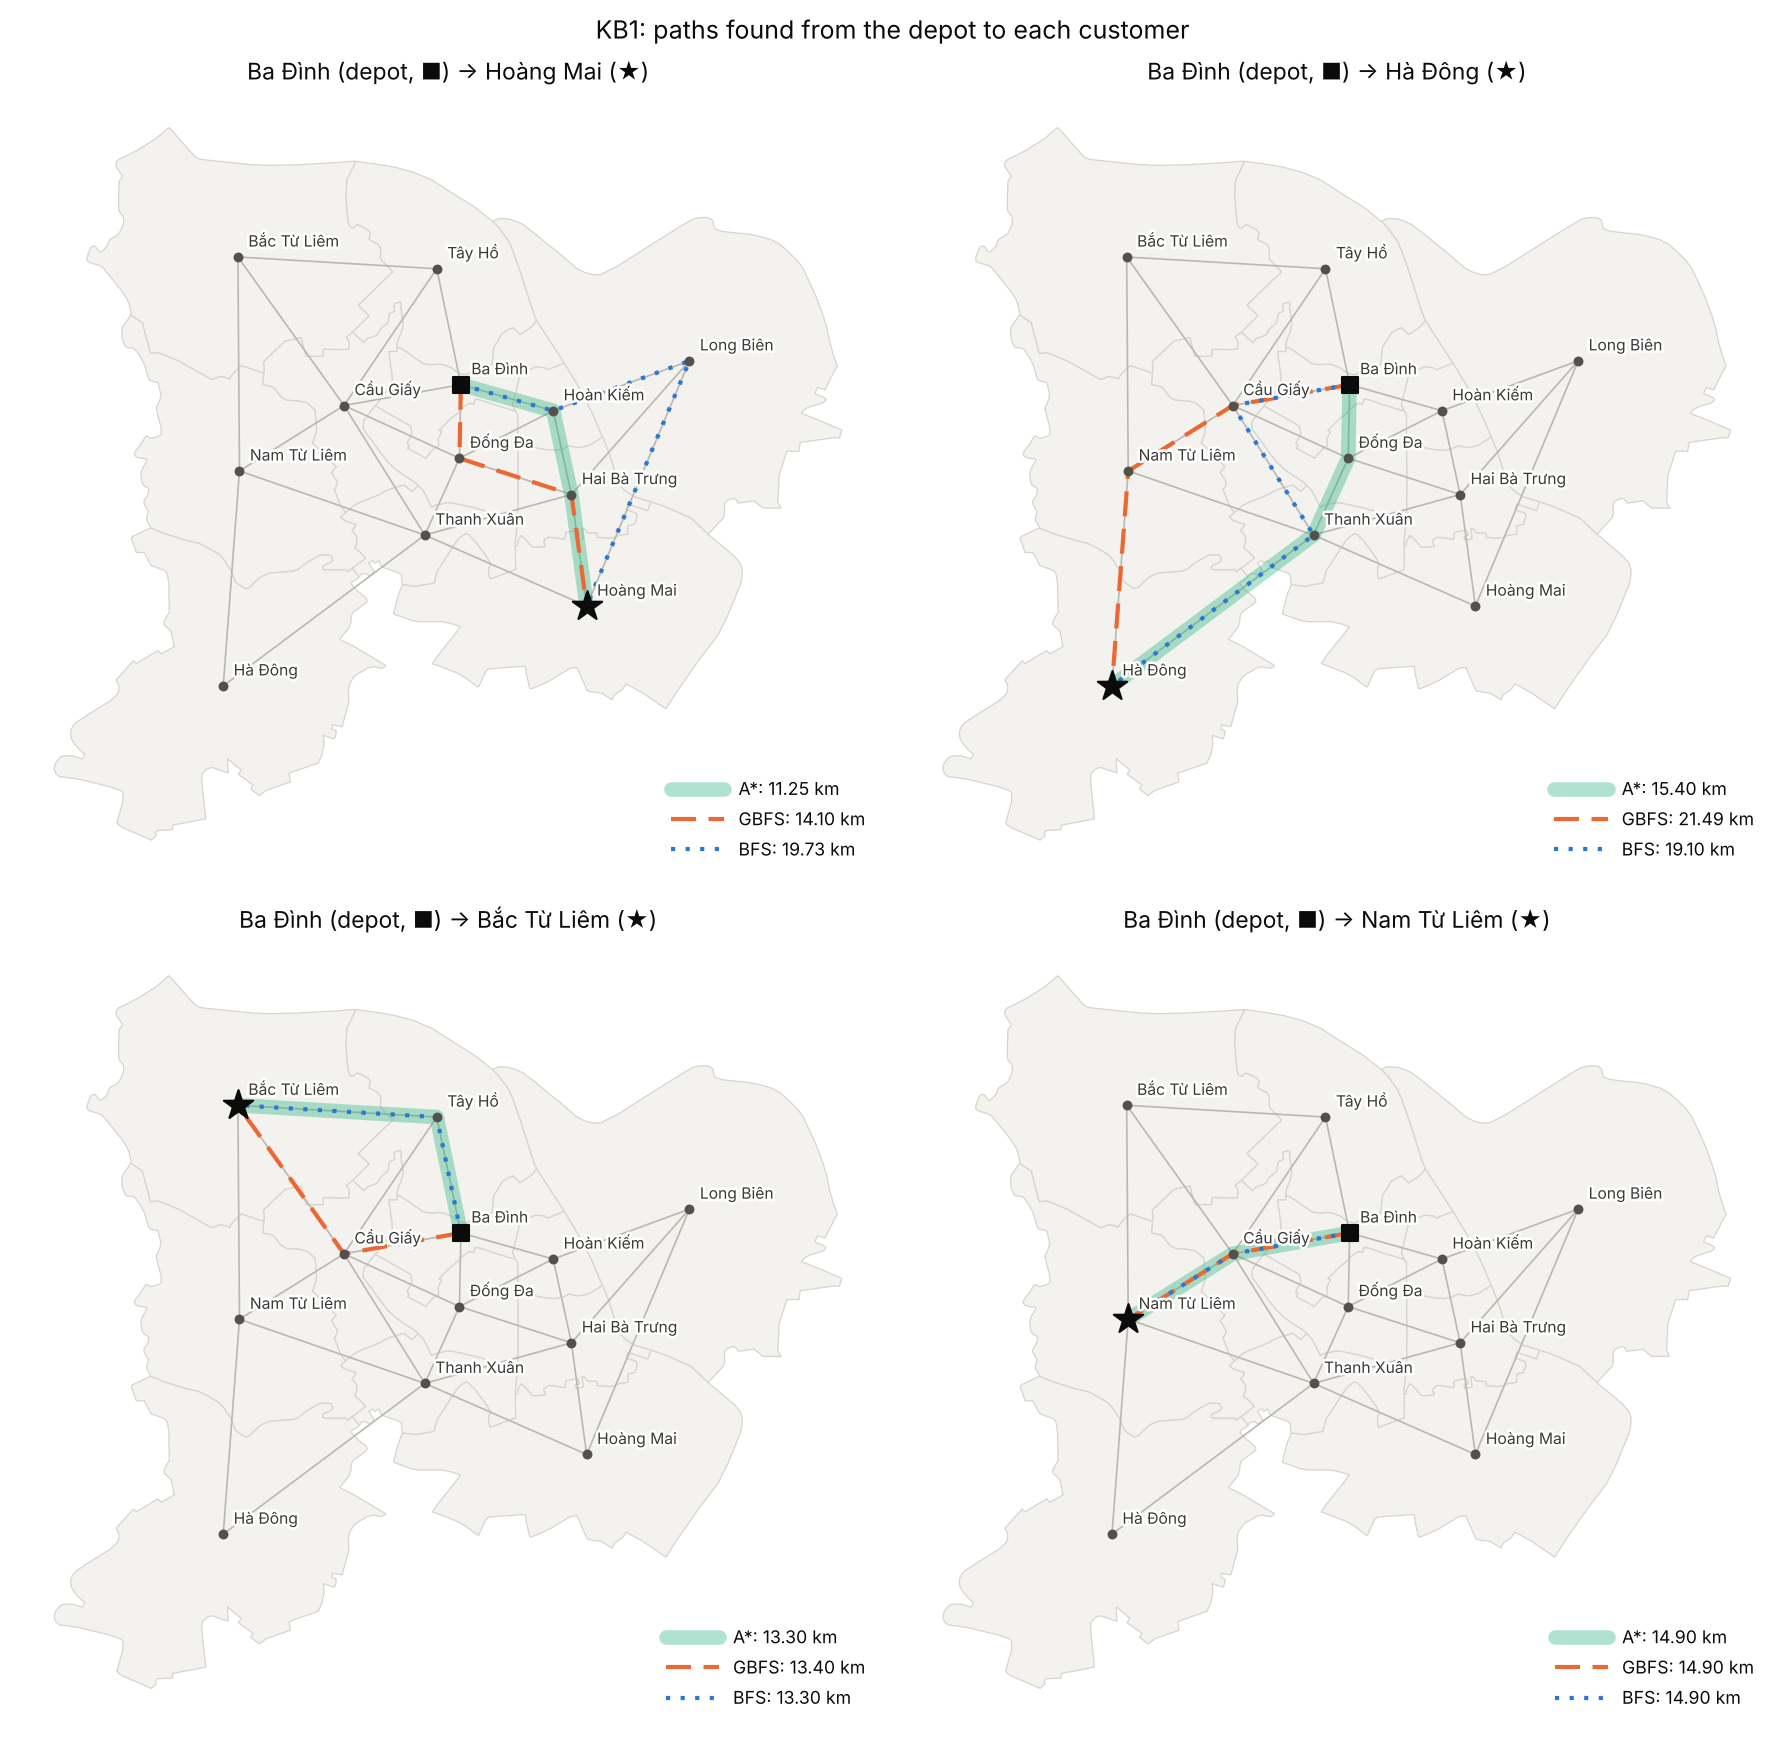
\includegraphics[width=1.0\linewidth,height=0.7\textheight,keepaspectratio]{figures/hinh1_kb1_duong_di.png}
\caption{Paths found by BFS, GBFS and A\* from the Ba Đình depot to the four customers.}
\end{figure}

\subsection{KB2: Depot in Every District}

A* is optimal for all 132 pairs and expands 52\% fewer nodes
than UCS (Table 17, Figures 3 and 4). With real road
distances, GBFS's optimality rate falls even below that of
BFS.

\begin{longtable}[]{@{}
  >{\raggedright\arraybackslash}p{(\columnwidth - 12\tabcolsep) * \real{0.1667}}
  >{\raggedright\arraybackslash}p{(\columnwidth - 12\tabcolsep) * \real{0.1833}}
  >{\raggedright\arraybackslash}p{(\columnwidth - 12\tabcolsep) * \real{0.1167}}
  >{\raggedright\arraybackslash}p{(\columnwidth - 12\tabcolsep) * \real{0.1167}}
  >{\raggedright\arraybackslash}p{(\columnwidth - 12\tabcolsep) * \real{0.1500}}
  >{\raggedright\arraybackslash}p{(\columnwidth - 12\tabcolsep) * \real{0.1500}}
  >{\raggedright\arraybackslash}p{(\columnwidth - 12\tabcolsep) * \real{0.1167}}@{}}
\caption{KB2 summary (132 depot--customer
pairs).}\tabularnewline
\toprule\noalign{}
\begin{minipage}[b]{\linewidth}\raggedright
Algorithm
\end{minipage} & \begin{minipage}[b]{\linewidth}\raggedright
Optimality rate (\%)
\end{minipage} & \begin{minipage}[b]{\linewidth}\raggedright
Mean excess (\%)
\end{minipage} & \begin{minipage}[b]{\linewidth}\raggedright
Max excess (\%)
\end{minipage} & \begin{minipage}[b]{\linewidth}\raggedright
Mean expanded nodes
\end{minipage} & \begin{minipage}[b]{\linewidth}\raggedright
Mean max frontier
\end{minipage} & \begin{minipage}[b]{\linewidth}\raggedright
Mean time (\(\mu\)s)
\end{minipage} \\
\midrule\noalign{}
\endfirsthead
\toprule\noalign{}
\begin{minipage}[b]{\linewidth}\raggedright
Algorithm
\end{minipage} & \begin{minipage}[b]{\linewidth}\raggedright
Optimality rate (\%)
\end{minipage} & \begin{minipage}[b]{\linewidth}\raggedright
Mean excess (\%)
\end{minipage} & \begin{minipage}[b]{\linewidth}\raggedright
Max excess (\%)
\end{minipage} & \begin{minipage}[b]{\linewidth}\raggedright
Mean expanded nodes
\end{minipage} & \begin{minipage}[b]{\linewidth}\raggedright
Mean max frontier
\end{minipage} & \begin{minipage}[b]{\linewidth}\raggedright
Mean time (\(\mu\)s)
\end{minipage} \\
\midrule\noalign{}
\endhead
\bottomrule\noalign{}
\endlastfoot
BFS & 84.8 & 5.37 & 101.9 & 6.00 & 5.34 & 6.7 \\
GBFS & 81.8 & 3.13 & 55.5 & 1.90 & 5.27 & 6.2 \\
A* & 100.0 & 0.00 & 0.0 & 2.87 & 5.48 & 9.7 \\
UCS & 100.0 & 0.00 & 0.0 & 6.00 & 5.96 & 12.4 \\
\end{longtable}

\begin{itemize}
\tightlist
\item
  \textbf{When BFS fails} (20/132 pairs), its path is 35.4\%
  longer on average; the worst case is +101.9\% (Hoàn Kiếm
  \(\rightarrow\) Long Biên \(\rightarrow\) Hoàng Mai).
\item
  \textbf{When GBFS fails} (24/132 pairs), its path is
  17.2\% longer on average; the worst case is +55.5\% (Hoàng
  Mai \(\rightarrow\) Thanh Xuân \(\rightarrow\) Đống Đa
  \(\rightarrow\) Ba Đình).
\item
  \textbf{Independent of depot location.} For all 12 depot
  locations, GBFS expands no more nodes than A*, and A* no
  more than UCS; pair by pair, A* never expands more nodes
  than UCS (0/132), as predicted by Section 4.2.
\item
  \textbf{Why BFS and UCS always average exactly 6.00
  nodes.} Neither algorithm uses information about the goal,
  so the order in which nodes are removed depends only on
  the depot. If the goal is the j-th node removed, j \(-\) 1
  nodes have been expanded; averaged over 11 goals this is
  (1 + 2 + \ldots{} + 11)/11 = 6. This is the cost of blind
  search; the drop from 6 to 2.87 is the saving due to the
  heuristic.
\item
  \textbf{Running time} is only a few microseconds and
  machine-dependent, so it is not used as primary evidence.
\end{itemize}

\begin{figure}[H]
\centering
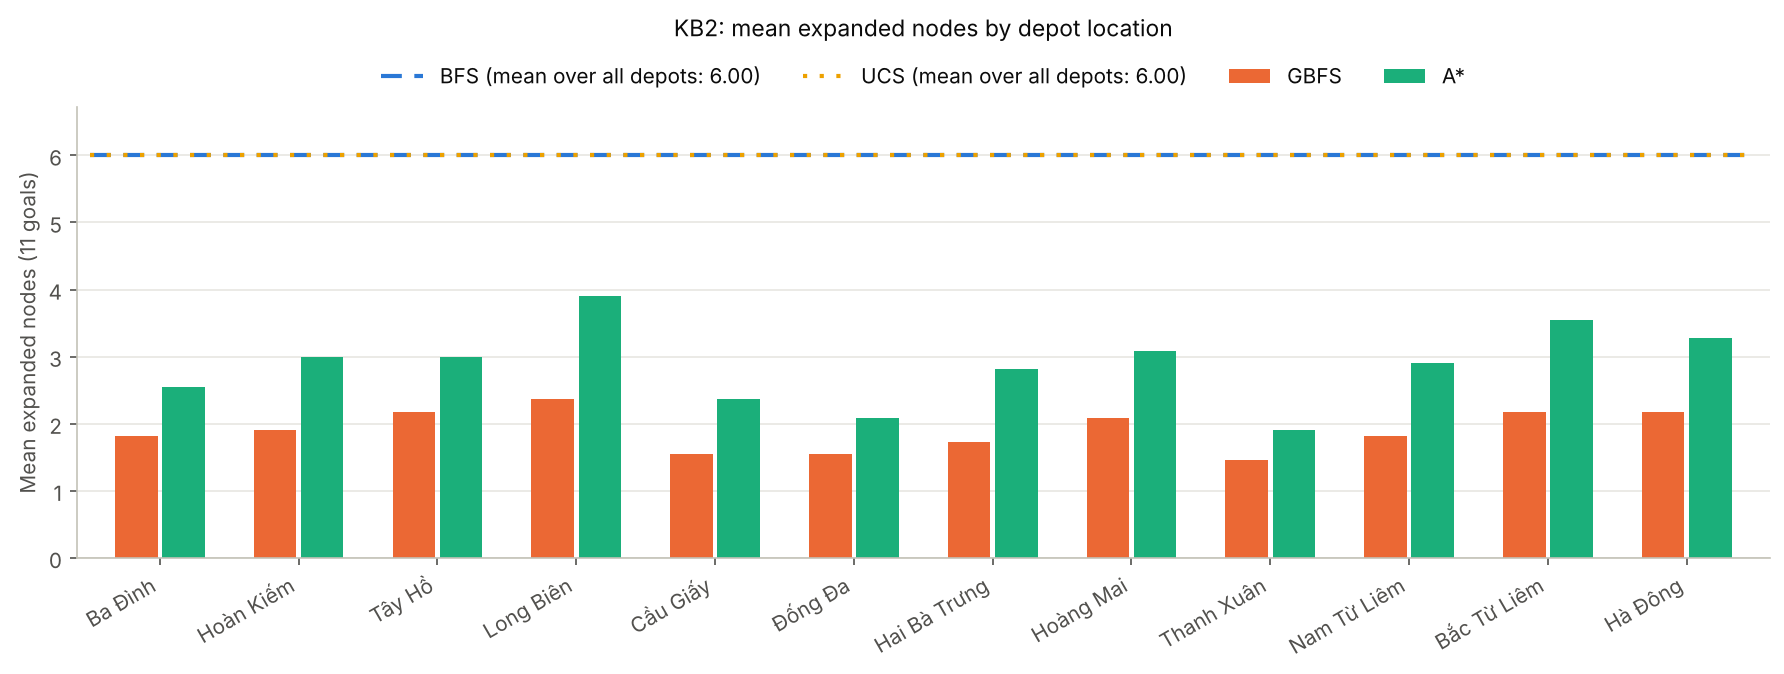
\includegraphics[width=1.0\linewidth,height=0.7\textheight,keepaspectratio]{figures/hinh2_kb2_node_theo_kho.png}
\caption{Mean expanded nodes by depot location.}
\end{figure}

\begin{figure}[H]
\centering
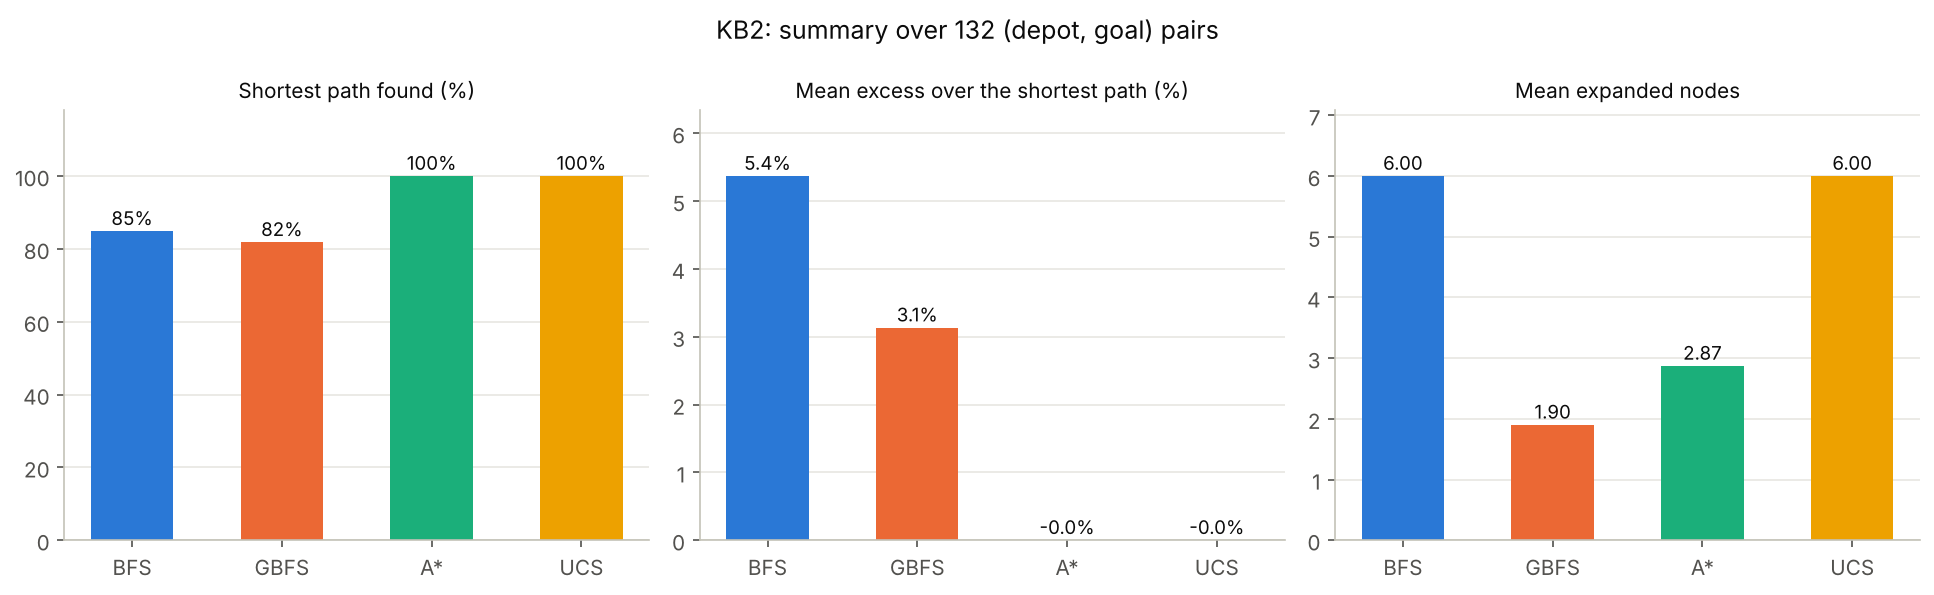
\includegraphics[width=1.0\linewidth,height=0.7\textheight,keepaspectratio]{figures/hinh3_kb2_tong_hop.png}
\caption{Optimality rate, mean excess and mean expanded nodes over 132 pairs.}
\end{figure}

\subsection{KB3: Road Tortuosity}

As the maximum tortuosity factor rises from 1.0 to 2.0, the
optimality rate of BFS falls from 81.8\% to 73.3\% and that
of GBFS from 84.8\% to 76.2\%; A* remains 100\% optimal, but
its expanded nodes rise from 2.02 to 2.88 (Table 18, Figure
5).

\begin{longtable}[]{@{}
  >{\raggedright\arraybackslash}p{(\columnwidth - 10\tabcolsep) * \real{0.1000}}
  >{\raggedright\arraybackslash}p{(\columnwidth - 10\tabcolsep) * \real{0.1667}}
  >{\raggedright\arraybackslash}p{(\columnwidth - 10\tabcolsep) * \real{0.1750}}
  >{\raggedright\arraybackslash}p{(\columnwidth - 10\tabcolsep) * \real{0.1750}}
  >{\raggedright\arraybackslash}p{(\columnwidth - 10\tabcolsep) * \real{0.1750}}
  >{\raggedright\arraybackslash}p{(\columnwidth - 10\tabcolsep) * \real{0.2083}}@{}}
\caption{KB3 results by maximum tortuosity factor
k.}\tabularnewline
\toprule\noalign{}
\begin{minipage}[b]{\linewidth}\raggedright
k
\end{minipage} & \begin{minipage}[b]{\linewidth}\raggedright
BFS optimal (\%)
\end{minipage} & \begin{minipage}[b]{\linewidth}\raggedright
GBFS optimal (\%)
\end{minipage} & \begin{minipage}[b]{\linewidth}\raggedright
BFS mean excess (\%)
\end{minipage} & \begin{minipage}[b]{\linewidth}\raggedright
GBFS mean excess (\%)
\end{minipage} & \begin{minipage}[b]{\linewidth}\raggedright
A* mean expanded nodes
\end{minipage} \\
\midrule\noalign{}
\endfirsthead
\toprule\noalign{}
\begin{minipage}[b]{\linewidth}\raggedright
k
\end{minipage} & \begin{minipage}[b]{\linewidth}\raggedright
BFS optimal (\%)
\end{minipage} & \begin{minipage}[b]{\linewidth}\raggedright
GBFS optimal (\%)
\end{minipage} & \begin{minipage}[b]{\linewidth}\raggedright
BFS mean excess (\%)
\end{minipage} & \begin{minipage}[b]{\linewidth}\raggedright
GBFS mean excess (\%)
\end{minipage} & \begin{minipage}[b]{\linewidth}\raggedright
A* mean expanded nodes
\end{minipage} \\
\midrule\noalign{}
\endhead
\bottomrule\noalign{}
\endlastfoot
1.00 & 81.8 & 84.8 & 5.57 & 1.66 & 2.02 \\
1.25 & 79.3 & 82.4 & 5.60 & 1.84 & 2.31 \\
1.50 & 77.5 & 80.7 & 6.64 & 2.36 & 2.53 \\
2.00 & 73.3 & 76.2 & 8.31 & 3.91 & 2.88 \\
\end{longtable}

BFS and GBFS do not use edge lengths while searching, so
their paths and node counts do not change with k (BFS 6.00,
GBFS 1.90); the true shortest path does change with edge
lengths, however, so they deviate from it more and more
often. UCS always expands 6.00 nodes.

\textbf{Comparison with real data.} Real roads are on
average about 1.5 times the straight-line distance, which
matches k = 2.0 in KB3 (mean factor (1 + 2)/2 = 1.5). At
that level, KB3 predicts 2.88 expanded nodes for A*; the
real road data in KB2 give 2.87.

\begin{figure}[H]
\centering
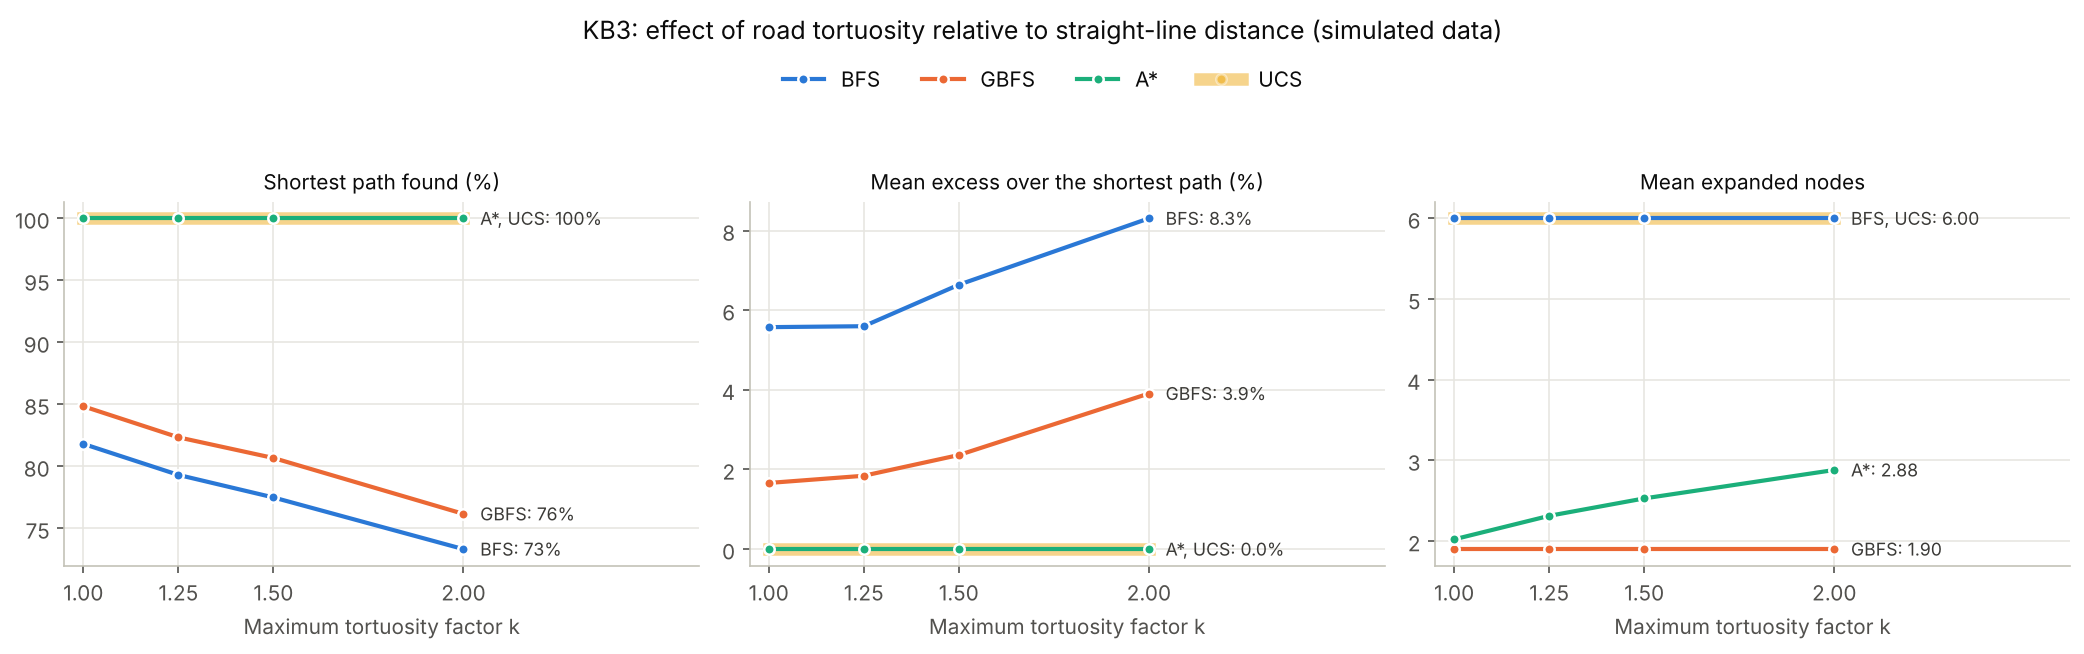
\includegraphics[width=1.0\linewidth,height=0.7\textheight,keepaspectratio]{figures/hinh4_kb3_do_nhay.png}
\caption{Sensitivity of the algorithms to the tortuosity factor k (simulated data).}
\end{figure}

\subsection{KB4: Scaling Up the Map}

\textbf{Map generation.} Points are scattered uniformly at
constant density (about 9 km\(^2\) per node); edges form a
Delaunay triangulation, which resembles a planar road
network; each edge length is the straight-line distance
multiplied by a random factor in {[}1; 1.25{]}. The ground
truth is UCS.

The expanded-node counts of BFS and UCS nearly coincide and
grow roughly in proportion to map size; the ratio of A* to
UCS falls from 32\% (25 nodes) to 21\% (800 nodes) (Figure
6). Meanwhile, the optimality rates of BFS and GBFS drop
sharply as the map grows (Table 19): the more legs a path
has, the more chances there are to choose wrongly. The
excess of GBFS levels off around 11\%, while that of BFS
keeps rising to nearly 50\%. A* and UCS are 100\% optimal at
every size.

\begin{figure}[H]
\centering
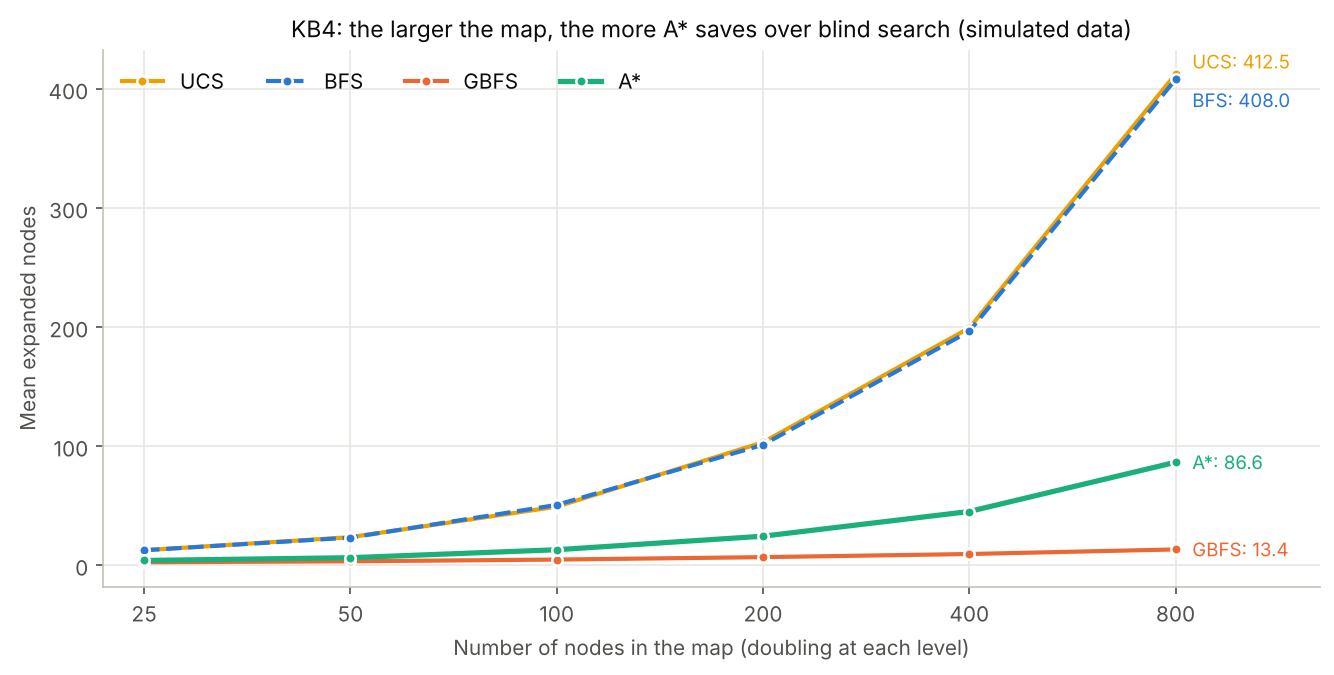
\includegraphics[width=1.0\linewidth,height=0.7\textheight,keepaspectratio]{figures/hinh5_kb4_tang_quy_mo.png}
\caption{Mean expanded nodes by map size (simulated data). Values from 25 to 800 nodes: UCS 12.7 $\rightarrow$ 412.5; BFS 12.7 $\rightarrow$ 408.0; A\* 4.1 $\rightarrow$ 86.6; GBFS 2.6 $\rightarrow$ 13.4.}
\end{figure}

\begin{longtable}[]{@{}
  >{\raggedright\arraybackslash}p{(\columnwidth - 8\tabcolsep) * \real{0.1157}}
  >{\raggedright\arraybackslash}p{(\columnwidth - 8\tabcolsep) * \real{0.1983}}
  >{\raggedright\arraybackslash}p{(\columnwidth - 8\tabcolsep) * \real{0.2066}}
  >{\raggedright\arraybackslash}p{(\columnwidth - 8\tabcolsep) * \real{0.2314}}
  >{\raggedright\arraybackslash}p{(\columnwidth - 8\tabcolsep) * \real{0.2479}}@{}}
\caption{Path quality of BFS and GBFS by map
size.}\tabularnewline
\toprule\noalign{}
\begin{minipage}[b]{\linewidth}\raggedright
Nodes
\end{minipage} & \begin{minipage}[b]{\linewidth}\raggedright
BFS optimal (\%)
\end{minipage} & \begin{minipage}[b]{\linewidth}\raggedright
GBFS optimal (\%)
\end{minipage} & \begin{minipage}[b]{\linewidth}\raggedright
BFS mean excess (\%)
\end{minipage} & \begin{minipage}[b]{\linewidth}\raggedright
GBFS mean excess (\%)
\end{minipage} \\
\midrule\noalign{}
\endfirsthead
\toprule\noalign{}
\begin{minipage}[b]{\linewidth}\raggedright
Nodes
\end{minipage} & \begin{minipage}[b]{\linewidth}\raggedright
BFS optimal (\%)
\end{minipage} & \begin{minipage}[b]{\linewidth}\raggedright
GBFS optimal (\%)
\end{minipage} & \begin{minipage}[b]{\linewidth}\raggedright
BFS mean excess (\%)
\end{minipage} & \begin{minipage}[b]{\linewidth}\raggedright
GBFS mean excess (\%)
\end{minipage} \\
\midrule\noalign{}
\endhead
\bottomrule\noalign{}
\endlastfoot
25 & 48.3 & 57.3 & 18.5 & 6.6 \\
50 & 40.0 & 51.7 & 20.0 & 6.7 \\
100 & 26.0 & 33.3 & 28.9 & 10.2 \\
200 & 14.3 & 18.0 & 32.8 & 10.6 \\
400 & 8.0 & 10.3 & 36.8 & 11.0 \\
800 & 5.0 & 5.0 & 49.8 & 10.8 \\
\end{longtable}

\section{Discussion}

\subsection{Choosing an Algorithm}

No algorithm suits every situation, but for delivery routing
on a weighted map, A* is the most sensible default (Table
20).

\begin{longtable}[]{@{}
  >{\raggedright\arraybackslash}p{(\columnwidth - 6\tabcolsep) * \real{0.1917}}
  >{\raggedright\arraybackslash}p{(\columnwidth - 6\tabcolsep) * \real{0.2917}}
  >{\raggedright\arraybackslash}p{(\columnwidth - 6\tabcolsep) * \real{0.2583}}
  >{\raggedright\arraybackslash}p{(\columnwidth - 6\tabcolsep) * \real{0.2583}}@{}}
\caption{The three algorithms in a delivery
context.}\tabularnewline
\toprule\noalign{}
\begin{minipage}[b]{\linewidth}\raggedright
Criterion
\end{minipage} & \begin{minipage}[b]{\linewidth}\raggedright
BFS
\end{minipage} & \begin{minipage}[b]{\linewidth}\raggedright
GBFS
\end{minipage} & \begin{minipage}[b]{\linewidth}\raggedright
A*
\end{minipage} \\
\midrule\noalign{}
\endfirsthead
\toprule\noalign{}
\begin{minipage}[b]{\linewidth}\raggedright
Criterion
\end{minipage} & \begin{minipage}[b]{\linewidth}\raggedright
BFS
\end{minipage} & \begin{minipage}[b]{\linewidth}\raggedright
GBFS
\end{minipage} & \begin{minipage}[b]{\linewidth}\raggedright
A*
\end{minipage} \\
\midrule\noalign{}
\endhead
\bottomrule\noalign{}
\endlastfoot
Principle & Expands level by level, from near to far from
the depot & Prefers the node that looks closest to the goal
& Weighs both the cost so far g(n) and the estimated
remaining cost h(n) \\
Path quality & Fewest legs; shortest only when all edges are
equal & Not guaranteed to be shortest & Always shortest with
a consistent heuristic \\
Search cost & High: spreads evenly, no sense of direction &
Lowest when the heuristic points the right way & Low; higher
than GBFS but far lower than UCS \\
Suited to & Simple uniform-cost networks (warehouse aisles,
grids); baseline & Quick preliminary routes when longer
trips are acceptable & Routing between depot and delivery
points with distance or time weights \\
Main limitation & Ignores edge lengths; memory-hungry on
large maps & Misled by detours, dead ends, one-way streets &
Needs correct weights and heuristic; does not order multiple
stops \\
\end{longtable}

GBFS is ``fast'' in the sense of expanding few nodes, not in
the sense of producing shorter routes. On the 12-district
map with real roads, A* expands about one more node per
search than GBFS (2.87 vs 1.90) but always finds the
shortest path, while GBFS fails on 24 of 132 pairs. On
800-node graphs, A* expands about 6.5 times as many nodes as
GBFS but still only 21\% of what UCS expands. If even faster
search is needed with bounded error, weighted A* (f = g +
w\(\cdot\)h) is worth considering.

\subsection{Application to Real Delivery}

\begin{itemize}
\tightlist
\item
  \textbf{Leg-by-leg routing (micro-routing).} A* finds the
  route from the depot to a delivery point or between two
  consecutive delivery points. To minimise distance, the
  weight is km; to minimise time, the weight is expected
  travel time, provided suitable data exist and the
  heuristic still never overestimates.
\item
  \textbf{Ordering many stops (macro-routing).} A* does not
  decide the order in which to visit many addresses. That
  requires methods for the Vehicle Routing Problem or
  metaheuristics such as Genetic Algorithms or Ant Colony
  Optimization {[}6{]}, {[}7{]}; A* then computes the route
  between consecutive stops.
\item
  \textbf{Changing traffic.} When congestion occurs, the
  system updates edge weights and searches again; methods
  such as D* Lite reuse the results of the previous search
  {[}5{]}.
\end{itemize}

\subsection{Design Trade-offs}

Each modelling choice in this study trades some realism for
a clearer, fully verifiable comparison of the three
algorithms (Table 21).

\begin{longtable}[]{@{}
  >{\raggedright\arraybackslash}p{(\columnwidth - 6\tabcolsep) * \real{0.2083}}
  >{\raggedright\arraybackslash}p{(\columnwidth - 6\tabcolsep) * \real{0.3000}}
  >{\raggedright\arraybackslash}p{(\columnwidth - 6\tabcolsep) * \real{0.2167}}
  >{\raggedright\arraybackslash}p{(\columnwidth - 6\tabcolsep) * \real{0.2750}}@{}}
\caption{Design choices and what they trade.}\tabularnewline
\toprule\noalign{}
\begin{minipage}[b]{\linewidth}\raggedright
Design choice
\end{minipage} & \begin{minipage}[b]{\linewidth}\raggedright
What it gains
\end{minipage} & \begin{minipage}[b]{\linewidth}\raggedright
What it gives up
\end{minipage} & \begin{minipage}[b]{\linewidth}\raggedright
How the study handles it
\end{minipage} \\
\midrule\noalign{}
\endfirsthead
\toprule\noalign{}
\begin{minipage}[b]{\linewidth}\raggedright
Design choice
\end{minipage} & \begin{minipage}[b]{\linewidth}\raggedright
What it gains
\end{minipage} & \begin{minipage}[b]{\linewidth}\raggedright
What it gives up
\end{minipage} & \begin{minipage}[b]{\linewidth}\raggedright
How the study handles it
\end{minipage} \\
\midrule\noalign{}
\endhead
\bottomrule\noalign{}
\endlastfoot
One node per district (centroid) & A small graph whose every
result can be checked by hand and by exhaustive search &
Street-level detail; customers sit at centroids, not
addresses & KB4 extends the comparison to graphs of up to
800 nodes \\
Distance (km) as the cost & Admissible, consistent
straight-line heuristic & Travel time, congestion, one-way
streets & The same A* applies unchanged once weights become
times with a non-overestimating heuristic \\
Google Maps road lengths, raised to the straight-line
distance when shorter & Real tortuosity while keeping the
heuristic consistent & Exact values for 4 of the 24 edges
(Table 6) & KB3 shows the conclusions hold for tortuosity
from 1 to 2 \\
District boundaries before 1 July 2025 & Stable, published
centroids from dvhcvn and geoBoundaries & Alignment with the
current administrative map & Algorithms and conclusions do
not depend on boundaries \\
One customer per search & A clean comparison of the search
algorithms themselves & Stop ordering within one trip &
Ordering is a separate VRP layer above A* (Section 7.2) \\
Simulated graphs in KB3--KB4 & Control over map size and
road tortuosity & Hanoi-specific figures & Used for trends
only; real data are in KB1--KB2 \\
Expanded nodes as the main efficiency metric & A
machine-independent, reproducible measure & Wall-clock time
on tiny graphs & Running times are reported but not used to
rank algorithms \\
\end{longtable}

\section{Conclusion and Future Work}

\subsection{Conclusion}

All four hypotheses are supported by the data (Table 22),
and the answer to the research question is A*.

\begin{longtable}[]{@{}
  >{\raggedright\arraybackslash}p{(\columnwidth - 6\tabcolsep) * \real{0.0583}}
  >{\raggedright\arraybackslash}p{(\columnwidth - 6\tabcolsep) * \real{0.3833}}
  >{\raggedright\arraybackslash}p{(\columnwidth - 6\tabcolsep) * \real{0.1750}}
  >{\raggedright\arraybackslash}p{(\columnwidth - 6\tabcolsep) * \real{0.3833}}@{}}
\caption{Hypothesis testing results.}\tabularnewline
\toprule\noalign{}
\begin{minipage}[b]{\linewidth}\raggedright
\end{minipage} & \begin{minipage}[b]{\linewidth}\raggedright
Hypothesis
\end{minipage} & \begin{minipage}[b]{\linewidth}\raggedright
Result
\end{minipage} & \begin{minipage}[b]{\linewidth}\raggedright
Main evidence
\end{minipage} \\
\midrule\noalign{}
\endfirsthead
\toprule\noalign{}
\begin{minipage}[b]{\linewidth}\raggedright
\end{minipage} & \begin{minipage}[b]{\linewidth}\raggedright
Hypothesis
\end{minipage} & \begin{minipage}[b]{\linewidth}\raggedright
Result
\end{minipage} & \begin{minipage}[b]{\linewidth}\raggedright
Main evidence
\end{minipage} \\
\midrule\noalign{}
\endhead
\bottomrule\noalign{}
\endlastfoot
H1 & BFS has the fewest legs but is not the shortest in km &
Supported & KB2: optimal 84.8\%; when wrong, 35.4\% longer
on average, worst +102\%. KB4: optimality drops to 5\% at
800 nodes \\
H2 & GBFS expands the fewest nodes but does not guarantee
optimality & Supported & KB2: 1.90 nodes (fewest), optimal
81.8\%, below BFS. KB4: 13 nodes vs 87 for A* at 800 nodes,
but only 5\% optimal \\
H3 & A* is always shortest and expands far fewer nodes than
UCS & Supported & Optimal in 100\% of runs. KB2: 2.87 vs
6.00 nodes (52\% fewer). KB4: 21\% of UCS's nodes at 800
nodes \\
H4 & The more tortuous the roads, the more BFS and GBFS
fail; A* stays optimal but expands more nodes & Supported &
KB3: BFS 81.8\% \(\rightarrow\) 73.3\%, GBFS 84.8\%
\(\rightarrow\) 76.2\%; A* stays at 100\%, nodes 2.02
\(\rightarrow\) 2.88. Real road data give A* 2.87 nodes,
matching KB3's prediction \\
\end{longtable}

Key takeaways:

\begin{enumerate}
\def\labelenumi{\arabic{enumi}.}
\tightlist
\item
  On a weighted map, ``fewest legs'' does not mean
  ``shortest'': BFS can choose a river-crossing detour twice
  as long as the shortest path.
\item
  The heuristic is the main source of savings: from 6 nodes
  (blind search) to under 3 nodes on the 12-district map
  with real roads.
\item
  Relying on the heuristic alone (GBFS) is fast, but its
  risk grows with map size; combining the heuristic with the
  cost so far (A*) keeps both advantages.
\item
  The conclusions do not depend on depot location (KB2) and
  become stronger as the map grows (KB4).
\end{enumerate}

\subsection{Future Work}

\begin{enumerate}
\def\labelenumi{\arabic{enumi}.}
\tightlist
\item
  Replace district centroids with a detailed road network
  (intersections and individual streets) from OpenStreetMap,
  including one-way streets.
\item
  Switch the cost from distance to time-of-day travel time,
  with a heuristic that still never overestimates.
\item
  Solve multi-stop delivery within one trip: order the stops
  with VRP methods or metaheuristics, then use A* for each
  leg.
\item
  Replan routes after traffic incidents with D* Lite and
  compare against re-running A* from scratch.
\item
  Test weighted A* (f = g + w\(\cdot\)h) to measure the
  trade-off between expanded nodes and path length.
\end{enumerate}

\section*{References}
\addcontentsline{toc}{section}{References}

{[}1{]} Google, Temasek and Bain \& Company, \emph{e-Conomy
SEA 2024}, Nov.~2024. {[}Online{]}. Available:
https://economysea.withgoogle.com

{[}2{]} S. J. Russell and P. Norvig, \emph{Artificial
Intelligence: A Modern Approach}, 4th ed.~Hoboken, NJ, USA:
Pearson, 2020.

{[}3{]} E. W. Dijkstra, ``A note on two problems in
connexion with graphs,'' \emph{Numerische Mathematik},
vol.~1, pp.~269--271, 1959, doi: 10.1007/BF01386390.

{[}4{]} P. E. Hart, N. J. Nilsson, and B. Raphael, ``A
formal basis for the heuristic determination of minimum cost
paths,'' \emph{IEEE Trans. Syst. Sci. Cybern.}, vol.~4, no.
2, pp.~100--107, 1968, doi: 10.1109/TSSC.1968.300136.

{[}5{]} S. Koenig and M. Likhachev, ``D* Lite,'' in
\emph{Proc. 18th AAAI Conf. Artif. Intell. (AAAI-02)}, 2002,
pp.~476--483.

{[}6{]} P. Toth and D. Vigo, Eds., \emph{Vehicle Routing:
Problems, Methods, and Applications}, 2nd ed.~Philadelphia,
PA, USA: SIAM, 2014., doi: 10.1137/1.9781611973594.

{[}7{]} R. Jazemi, E. Alidadiani, K. Ahn, and J. Jang, ``A
review of literature on vehicle routing problems of
last-mile delivery in urban areas,'' \emph{Applied
Sciences}, vol.~13, no. 24, Art. no. 13015, 2023, doi:
10.3390/app132413015.

{[}8{]} H.-S. Dao, ``dvhcvn: Vietnamese administrative
units,'' GitHub repository. {[}Online{]}. Available:
https://github.com/daohoangson/dvhcvn (data dated Mar.~1,
2025).

{[}9{]} D. Runfola \emph{et al.}, ``geoBoundaries: A global
database of political administrative boundaries,''
\emph{PLoS ONE}, vol.~15, no. 4, Art. no. e0231866, 2020,
doi: 10.1371/journal.pone.0231866.

{[}10{]} ``Diện mạo 9 cầu bắc qua sông Hồng'' {[}Nine
bridges across the Red River{]}, \emph{VnExpress}, Oct.~8,
2024. {[}Online{]}. Available:
https://vnexpress.net/9-cau-bac-qua-song-hong-4800203.html

{[}11{]} ``Top 7 cây cầu trọng yếu của Thủ đô Hà Nội''
{[}Top 7 key bridges of Hanoi{]}, \emph{Toplist}.
{[}Online{]}. Available:
https://toplist.vn/top-list/cay-cau-trong-yeu-cua-thu-do-ha-noi-284.htm

\appendix
\section*{Appendix}
\addcontentsline{toc}{section}{Appendix}

\subsection*{Appendix A. Centroids of the 12 Districts}
\addcontentsline{toc}{subsection}{Appendix A. Centroids of the 12 Districts}

The origin of (x, y) is the south-west corner of the
12-district area in UTM zone 48N.

\begin{longtable}[]{@{}
  >{\raggedright\arraybackslash}p{(\columnwidth - 12\tabcolsep) * \real{0.0909}}
  >{\raggedright\arraybackslash}p{(\columnwidth - 12\tabcolsep) * \real{0.1570}}
  >{\raggedright\arraybackslash}p{(\columnwidth - 12\tabcolsep) * \real{0.1901}}
  >{\raggedright\arraybackslash}p{(\columnwidth - 12\tabcolsep) * \real{0.1736}}
  >{\raggedright\arraybackslash}p{(\columnwidth - 12\tabcolsep) * \real{0.1240}}
  >{\raggedright\arraybackslash}p{(\columnwidth - 12\tabcolsep) * \real{0.1240}}
  >{\raggedright\arraybackslash}p{(\columnwidth - 12\tabcolsep) * \real{0.1405}}@{}}
\caption{Centroids of Hanoi's 12 urban districts (boundaries
before 1 July 2025).}\tabularnewline
\toprule\noalign{}
\begin{minipage}[b]{\linewidth}\raggedright
Code
\end{minipage} & \begin{minipage}[b]{\linewidth}\raggedright
District
\end{minipage} & \begin{minipage}[b]{\linewidth}\raggedright
Longitude
\end{minipage} & \begin{minipage}[b]{\linewidth}\raggedright
Latitude
\end{minipage} & \begin{minipage}[b]{\linewidth}\raggedright
x (km)
\end{minipage} & \begin{minipage}[b]{\linewidth}\raggedright
y (km)
\end{minipage} & \begin{minipage}[b]{\linewidth}\raggedright
Area (km\(^2\))
\end{minipage} \\
\midrule\noalign{}
\endfirsthead
\toprule\noalign{}
\begin{minipage}[b]{\linewidth}\raggedright
Code
\end{minipage} & \begin{minipage}[b]{\linewidth}\raggedright
District
\end{minipage} & \begin{minipage}[b]{\linewidth}\raggedright
Longitude
\end{minipage} & \begin{minipage}[b]{\linewidth}\raggedright
Latitude
\end{minipage} & \begin{minipage}[b]{\linewidth}\raggedright
x (km)
\end{minipage} & \begin{minipage}[b]{\linewidth}\raggedright
y (km)
\end{minipage} & \begin{minipage}[b]{\linewidth}\raggedright
Area (km\(^2\))
\end{minipage} \\
\midrule\noalign{}
\endhead
\bottomrule\noalign{}
\endlastfoot
001 & Ba Đình & 105.826699 & 21.036197 & 12.899 & 14.376 &
9.09 \\
002 & Hoàn Kiếm & 105.853811 & 21.028849 & 15.721 & 13.578 &
5.24 \\
003 & Tây Hồ & 105.819766 & 21.068239 & 12.161 & 17.919 &
23.40 \\
004 & Long Biên & 105.893984 & 21.042433 & 19.887 & 15.104 &
59.95 \\
005 & Cầu Giấy & 105.792284 & 21.030584 & 9.326 & 13.737 &
12.41 \\
006 & Đống Đa & 105.826156 & 21.015857 & 12.855 & 12.125 &
10.52 \\
007 & Hai Bà Trưng & 105.859037 & 21.005679 & 16.278 &
11.016 & 9.14 \\
008 & Hoàng Mai & 105.863349 & 20.974837 & 16.744 & 7.605 &
39.79 \\
009 & Thanh Xuân & 105.815860 & 20.994701 & 11.797 & 9.777 &
9.69 \\
019 & Nam Từ Liêm & 105.761423 & 21.012645 & 6.129 & 11.736
& 32.05 \\
021 & Bắc Từ Liêm & 105.761269 & 21.071765 & 6.082 & 18.279
& 45.32 \\
268 & Hà Đông & 105.756349 & 20.953309 & 5.633 & 5.166 &
49.49 \\
\end{longtable}

\subsection*{Appendix B. Lengths of the 24 Edges}
\addcontentsline{toc}{subsection}{Appendix B. Lengths of the 24 Edges}

\begin{longtable}[]{@{}
  >{\raggedright\arraybackslash}p{(\columnwidth - 6\tabcolsep) * \real{0.4333}}
  >{\raggedright\arraybackslash}p{(\columnwidth - 6\tabcolsep) * \real{0.1917}}
  >{\raggedright\arraybackslash}p{(\columnwidth - 6\tabcolsep) * \real{0.2417}}
  >{\raggedright\arraybackslash}p{(\columnwidth - 6\tabcolsep) * \real{0.1333}}@{}}
\caption{Straight-line distance between centroids and
measured road distance. Edges marked * are raised to the
straight-line distance in the experiments (Table
6).}\tabularnewline
\toprule\noalign{}
\begin{minipage}[b]{\linewidth}\raggedright
Edge
\end{minipage} & \begin{minipage}[b]{\linewidth}\raggedright
Crosses river
\end{minipage} & \begin{minipage}[b]{\linewidth}\raggedright
Straight-line (km)
\end{minipage} & \begin{minipage}[b]{\linewidth}\raggedright
Road (km)
\end{minipage} \\
\midrule\noalign{}
\endfirsthead
\toprule\noalign{}
\begin{minipage}[b]{\linewidth}\raggedright
Edge
\end{minipage} & \begin{minipage}[b]{\linewidth}\raggedright
Crosses river
\end{minipage} & \begin{minipage}[b]{\linewidth}\raggedright
Straight-line (km)
\end{minipage} & \begin{minipage}[b]{\linewidth}\raggedright
Road (km)
\end{minipage} \\
\midrule\noalign{}
\endhead
\bottomrule\noalign{}
\endlastfoot
Ba Đình -- Hoàn Kiếm * & no & 2.932 & 1.8 \\
Ba Đình -- Tây Hồ & no & 3.619 & 5.3 \\
Ba Đình -- Cầu Giấy & no & 3.630 & 6 \\
Ba Đình -- Đống Đa & no & 2.252 & 3.7 \\
Hoàn Kiếm -- Long Biên & yes & 4.437 & 6.8 \\
Hoàn Kiếm -- Đống Đa & no & 3.214 & 4.9 \\
Hoàn Kiếm -- Hai Bà Trưng * & no & 2.621 & 2.5 \\
Tây Hồ -- Cầu Giấy & no & 5.052 & 10 \\
Tây Hồ -- Bắc Từ Liêm & no & 6.090 & 8 \\
Long Biên -- Hai Bà Trưng & yes & 5.453 & 8 \\
Long Biên -- Hoàng Mai & yes & 8.131 & 10 \\
Cầu Giấy -- Đống Đa & no & 3.879 & 4.9 \\
Cầu Giấy -- Thanh Xuân & no & 4.667 & 5.4 \\
Cầu Giấy -- Nam Từ Liêm & no & 3.772 & 8.9 \\
Cầu Giấy -- Bắc Từ Liêm & no & 5.582 & 7.4 \\
Đống Đa -- Hai Bà Trưng & no & 3.598 & 4.7 \\
Đống Đa -- Thanh Xuân & no & 2.575 & 4 \\
Hai Bà Trưng -- Hoàng Mai & no & 3.443 & 5.7 \\
Hai Bà Trưng -- Thanh Xuân & no & 4.649 & 7.1 \\
Hoàng Mai -- Thanh Xuân & no & 5.404 & 9.8 \\
Thanh Xuân -- Nam Từ Liêm & no & 5.996 & 8.2 \\
Thanh Xuân -- Hà Đông * & no & 7.698 & 4.5 \\
Nam Từ Liêm -- Bắc Từ Liêm & no & 6.544 & 15 \\
Nam Từ Liêm -- Hà Đông * & no & 6.589 & 5.1 \\
\end{longtable}

\subsection*{Appendix C. Source Code}
\addcontentsline{toc}{subsection}{Appendix C. Source Code}

All source code (data download, graph construction, the four
algorithms, verification, scenarios KB1--KB4 and the
step-by-step traces) is in the notebook
\passthrough{\lstinline!finding\_route.ipynb!}, which runs
together with
\passthrough{\lstinline!real\_road\_data.csv!}. \emph{{[}TO
CHECK: add the group's GitHub or Google Drive link.{]}}
\end{document}
